\documentclass[9pt]{beamer}
%-----------------
% by Abolfazl Chaman Motlagh 
% September 2023
%-----------------

\usepackage[utf8]{inputenc}
\usepackage[brazil]{babel}
\usepackage{amssymb, amsmath, amsthm, amsfonts, amscd, graphicx, subfigure, array, multicol, setspace, caption, color,tikz}
\usetikzlibrary{intersections}
\usetikzlibrary{decorations.pathmorphing}
\usepackage{pifont} 
\usepackage{fix-cm}
\usepackage[style=alphabetic]{biblatex}
\addbibresource{ref.bib}
\usepackage{csquotes}

%Algorithms
\usepackage[ruled,lined,linesnumbered,commentsnumbered]{algorithm2e}

% Código
\newcommand{\code}[1]{\textcolor{white!25!black}{\texttt{#1}}}
\usepackage{listings}
%----------------------------------------------
\usecolortheme{beaver}
\usetheme{Frankfurt}
\setbeamercolor{section in head/foot}{bg=black}
\setbeamercolor{title}{fg=white, bg=black}
\setbeamercolor{frametitle}{fg=white,bg=black}
\setbeamercolor{block title}{fg=white,bg=black}
\setbeamercolor{item}{fg=gray}
\setbeamertemplate{navigation symbols}{}
\setbeamercovered{transparent}

%----------------------------------------------
\newcommand{\mysection}[1]{\section{#1} \def\sectionname{#1} \SectionFrame}
%----------------------------------------------
\newcommand{\Front}{\thispagestyle{empty}
\begin{frame}
    \begin{figure}  
        \centering
        
\includegraphics[width=0.3\textwidth]{Logos/Portada.jpg}
    \end{figure}
    \maketitle
\end{frame}
}

\newcommand{\overview}{\begin{frame}{Contenido}
\tableofcontents
\end{frame}}

\newcommand{\SectionFrame}{\begin{frame}{}
    \begin{center}
        {\fontsize{25pt}{36pt}\selectfont \thesection. \sectionname}
    \end{center}
\end{frame}}

\newcommand{\Ending}[1]{\begin{frame}{}
    \begin{center}
        {\fontsize{35pt}{36pt}\selectfont #1}
    \end{center}
\end{frame}}

\newcommand{\References}{\begin{frame}[allowframebreaks]{References}
    \printbibliography
\end{frame}}

\title[Title Short]{Estructuras de Datos Avanzadas 2024-1\\
                   \textbf{Conjuntos de discos independientes máximos totalmente dinámicos en tiempo poli-logarítmico.}}
\author[Name]{Adrián Aguilera Moreno \texorpdfstring{\\}{and}[1ex]
                     {\small{ \textbf{Profesora: Adriana Ramírez Vigueras}}}}
\institute[SUT]{Facultad de Ciencias UNAM}
\date[]{Octubre 2023}


\begin{document}
\Front
\overview
%----------------------------------------------
\mysection{Introducción}
\subsection{Resumen del problema.}
\begin{frame}{Intersecciones y el problema MIS}
  
  Descripción:
  
  \begin{itemize}[<+->]
  \item Intersectar objetos geométricos en $\mathbb{R}^n$ suele
    ser un problema muy estudiado en Geometría Computacional.
    \begin{figure}  
      \centering
      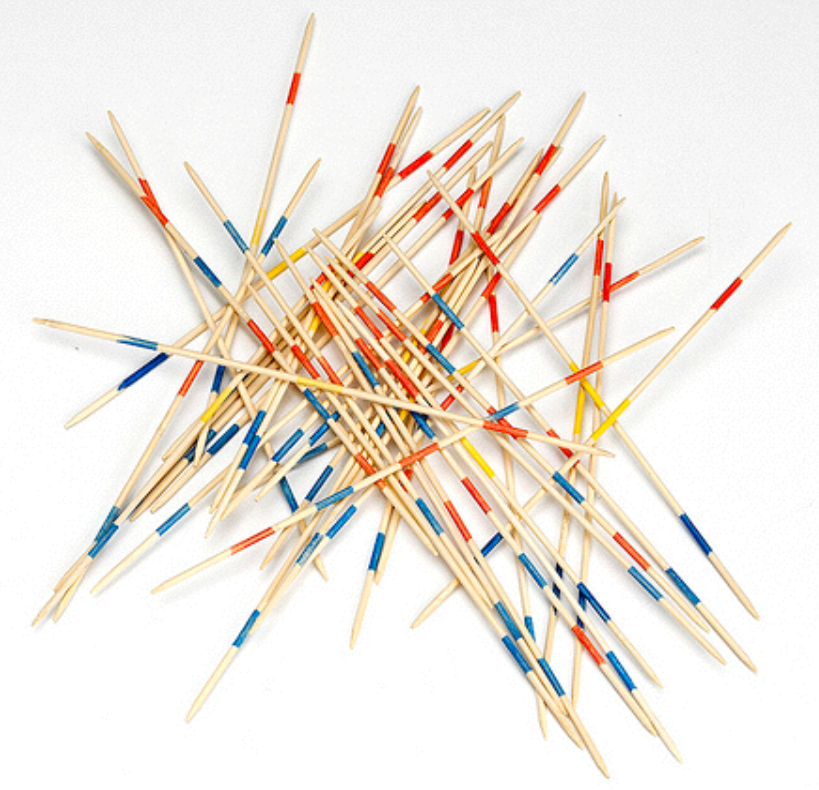
\includegraphics[width=0.25\textwidth]{./Images/Intersecciones.png}
    \end{figure}
    Podemos encontrar el número de intersecciones para segmentos en $\mathcal{O}(n \log n)$
    siendo sensible a su salida.
  \item ¿Podemos encontrar el máximo conjunto de objetos geométricos que no se intersecten?
  \item Encontrar el Conjunto Independiente Máximo (en adelante MIS) en una gráfica
    es uno de los problemas NP-Completo clásicos según Karp.
  \end{itemize}
\end{frame}

\begin{frame}{Colección de objetos geométricos.}
  
  Descripción:
  
  \begin{itemize}[<+->]
  \item Para una colección $\mathcal{L} = \{\ell_1, \dotsm, \ell_n\}$
    de objetos geométricos.
    \begin{figure}  
      \centering
      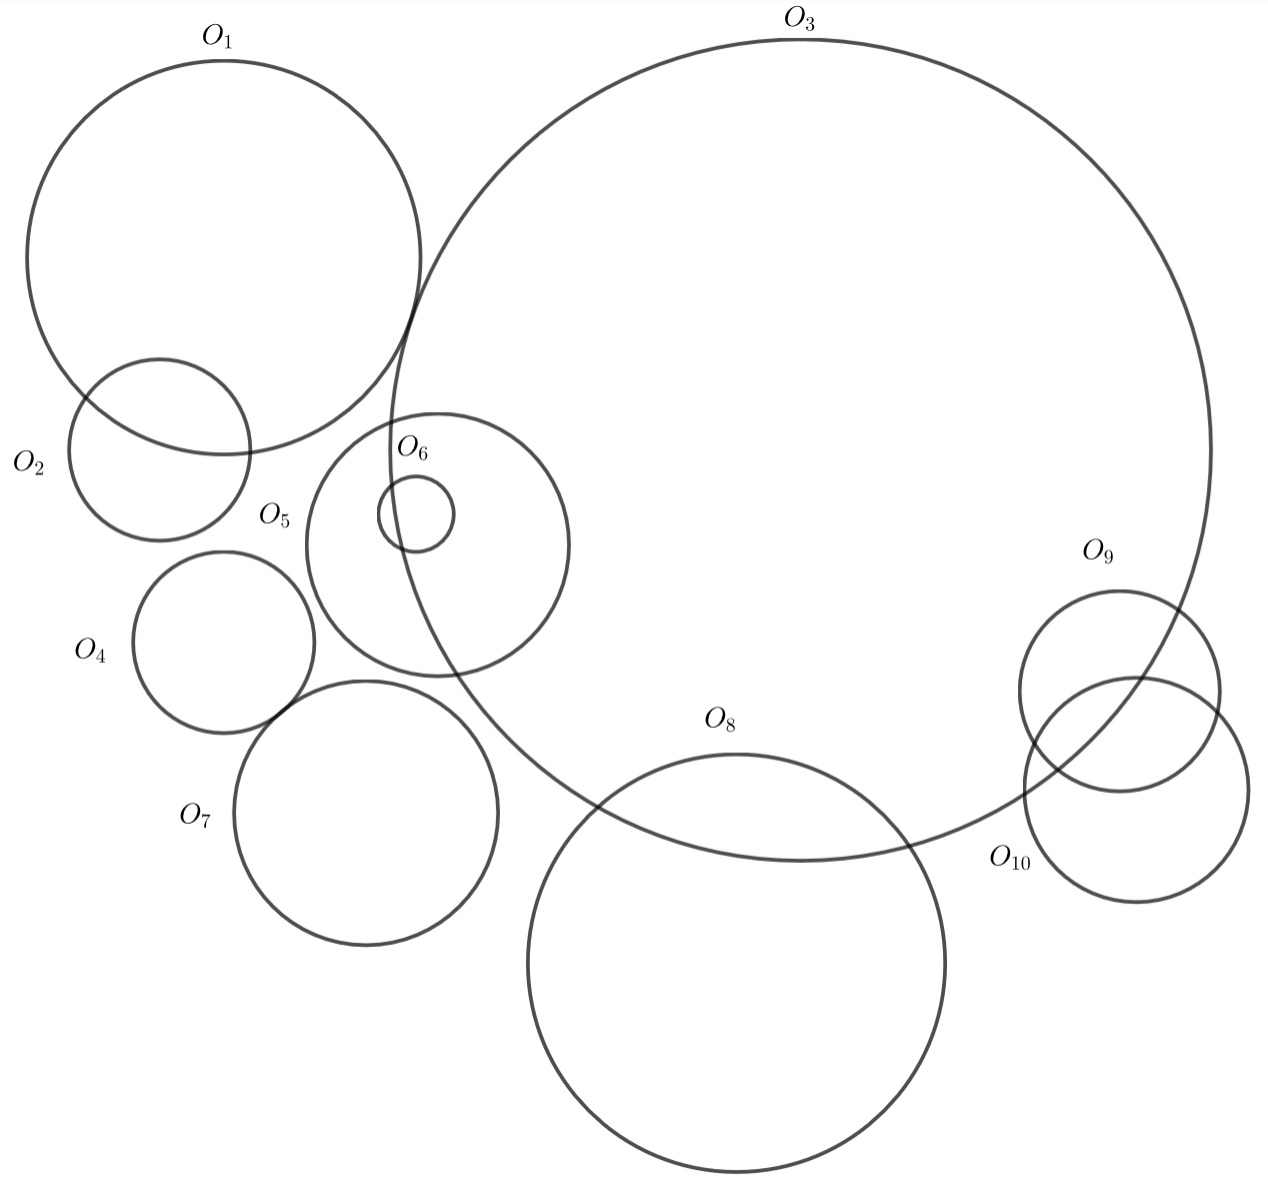
\includegraphics[width=0.7\textwidth]{./Images/Ejemplo01.png}
    \end{figure}
  \end{itemize}
\end{frame}

\begin{frame}{Dualidad.}
  
  \begin{itemize}[<+->]
  \item La gráfica de intersección $G_{\mathcal{L}} = (E_{\mathcal{L}},V_{\mathcal{L}})$
    de $\mathcal{L}$, cada objeto $\ell_i \in \mathcal{L}$ es representado por un vértice
    $v_i \in V_{\mathcal{L}}$ cualquier par $\ell_i \cap \ell_j \not= \varnothing$ se intersecta
    \textbf{SII} $(v_i, v_j) \in E_{\mathcal{L}}$.
    \begin{figure}  
      \centering
      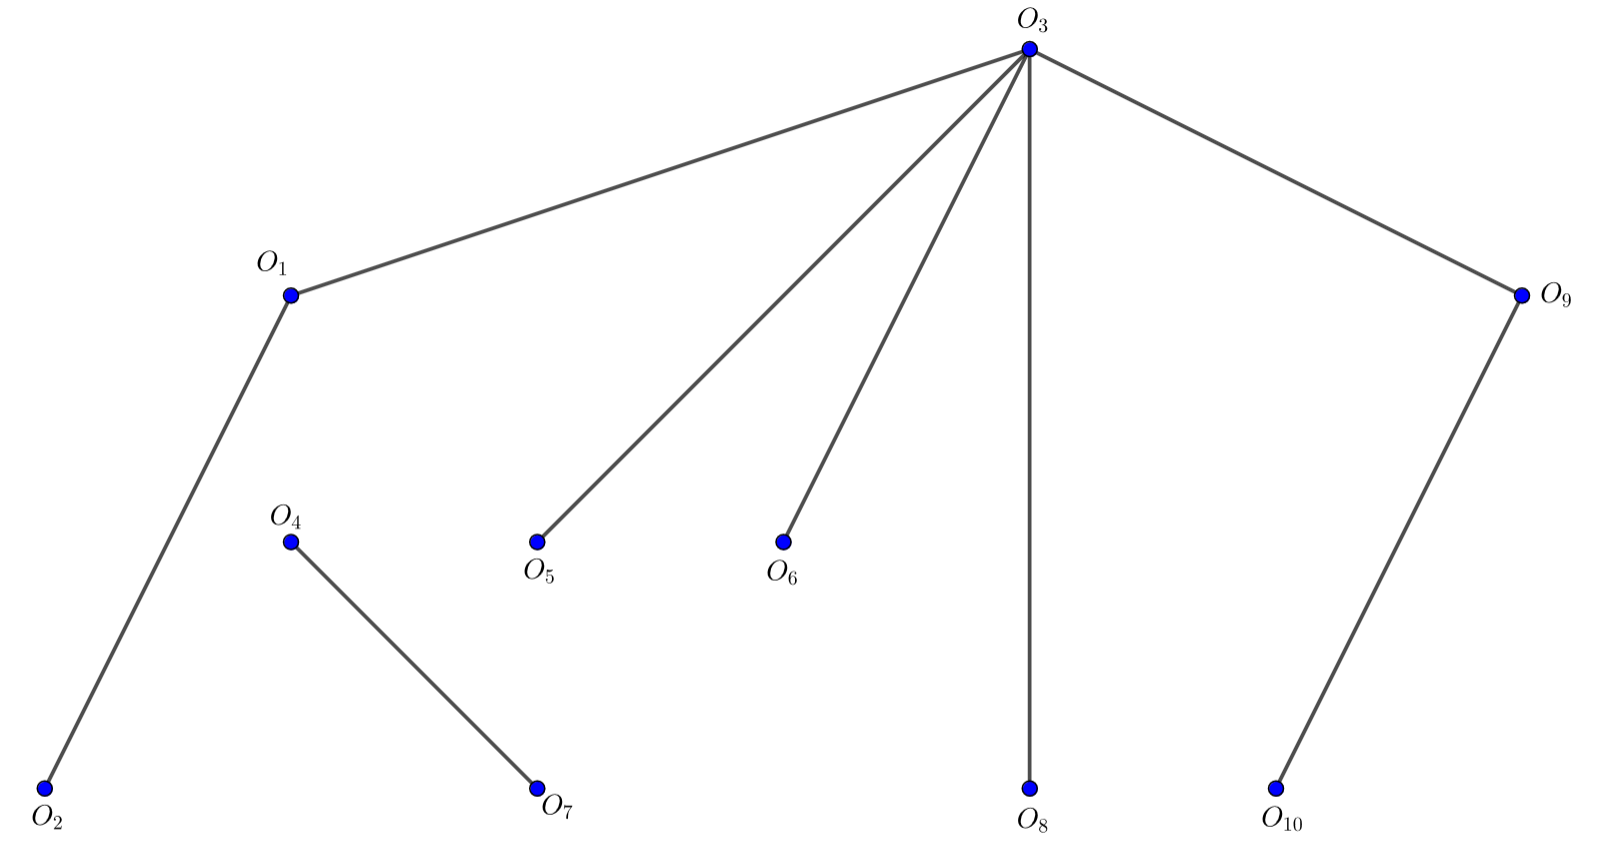
\includegraphics[width=0.8\textwidth]{./Images/Ejemplo02.png}
    \end{figure}
  \end{itemize}
\end{frame}

\begin{frame}{Conjuntos de discos independientes.}
  
  \begin{itemize}[<+->]
  \item Un conjunto independiente de $G_{\mathcal{L}}$ corresponde a un conjunto de objetos
    disjuntos por pares en $\mathcal{L}$.
    \begin{figure}  
      \centering
      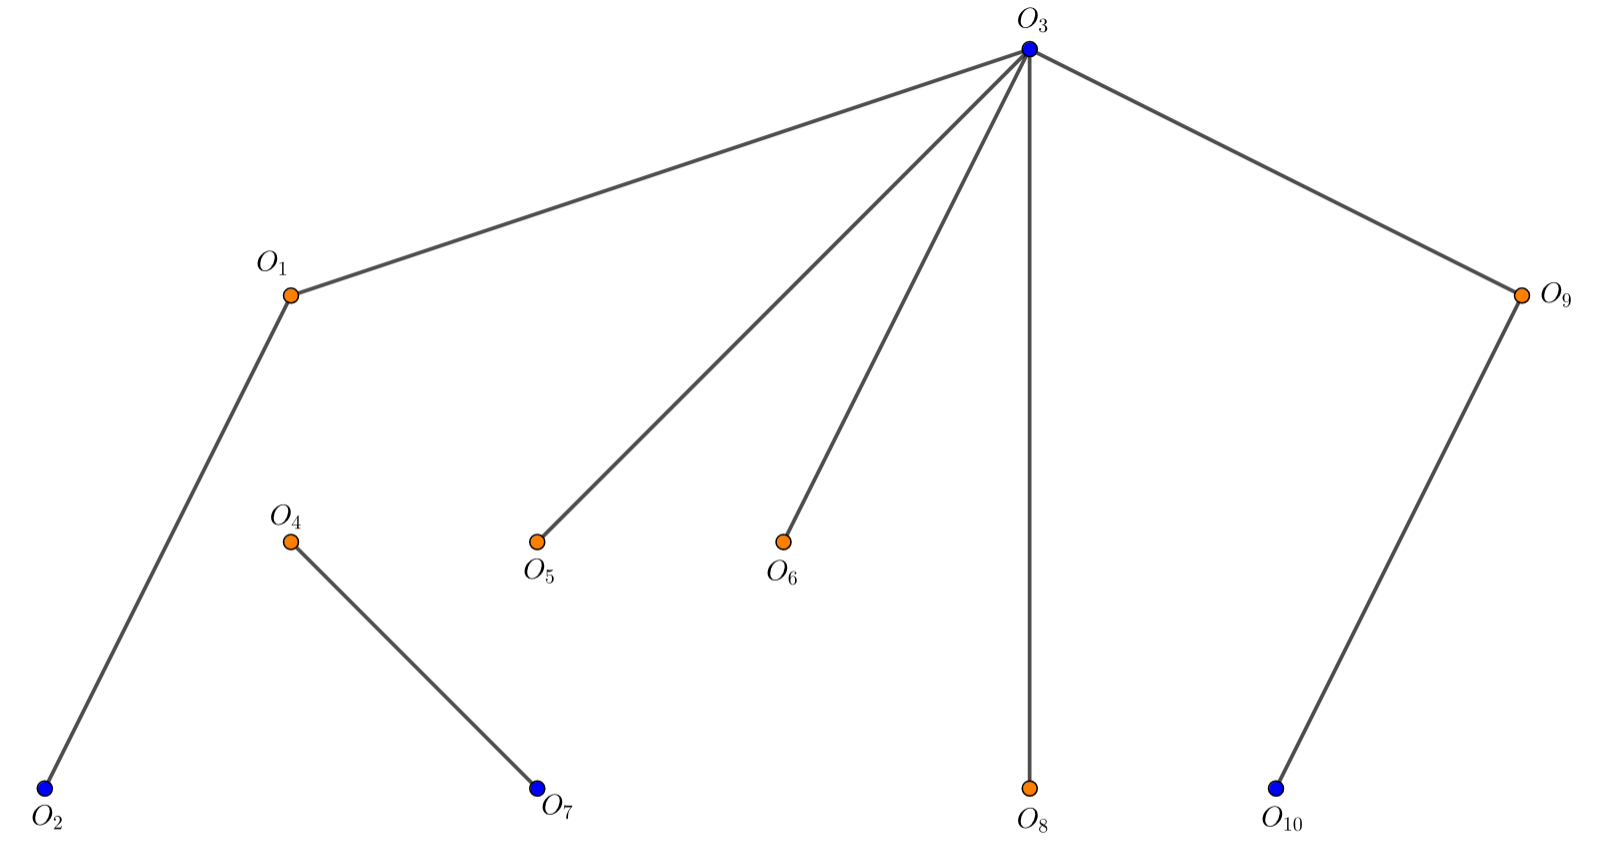
\includegraphics[width=0.8\textwidth]{./Images/Ejemplo03.png}
    \end{figure}
  \item Nuestro objetivo es mantener una estructura de datos que pueda mantener
    eficientemente un conjunto independiente $S \subseteq L$ cuyo tamaño sea una aproximación
    de factor constante del MIS de L en cualquier momento, con tiempos de actualización
    polilogarítmicos para inserciones y eliminaciones.
  \end{itemize}
  
\end{frame}


\begin{frame}{Antecedentes}
  
  Antecedentes:
  
  \begin{itemize}[<+->]
  \item En el 2022 Jean Cardinal et. al. crean el algoritmo \textit{offline} MIX para aproximar
    el conjunto independiente máximo de objetos gruesos en $\mathbb{R}^d$ con
    $d \in o(1)$ que se ejecuta en tiempo $\mathcal{O}(\alpha \log \alpha)$ con
    $\alpha$ el valor del máximo candidato a solución (en adelante OPT).
  \item La función MIX utiliza dos estructuras de datos, una de reciente creación
    llamada \textit{Estructura del vecino más cercano/lejano}, que se bassa en la
    idea del diagrama de Voronoi.
  \item Chan et. al. logran generalizar la estructura anterior a dimensiones superiores, siempre
    que sean constante respecto al número de objetos geométricos.
  \end{itemize}
\end{frame}

%----------------------------------------------
\mysection{Algoritmo MIX}
\subsection{Ejecución.}
\begin{frame}{Cuestión a abordar}
  \centering
  ¿Existe un algoritmo que para un conjunto dinámico, dado, de discos en
  el plano mantenga un conjunto independiente máximo aproximado de factor
  constante en tiempo de actualización poli-logarítmico?

  \begin{figure}  
    \centering
    
\includegraphics[width=0.6\textwidth]{./Images/autocuestionamiento.jpg}
  \end{figure}
\end{frame}


\begin{frame}{Ejecución}
  Supongamos el siguiente conjunto de discos unitarios en el plano
  \begin{figure}  
    \centering
    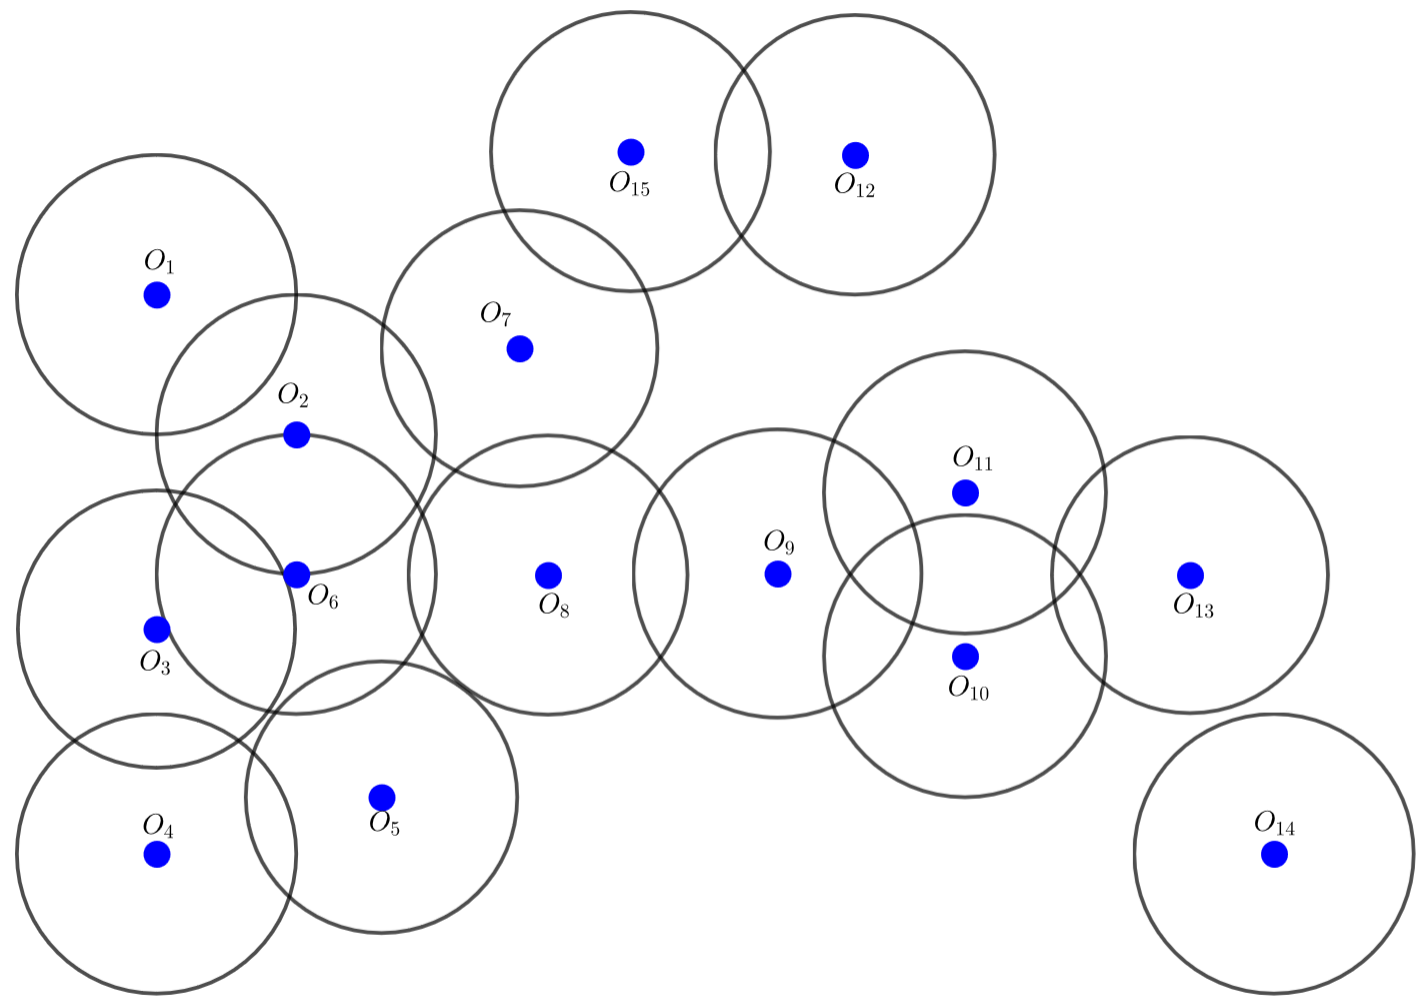
\includegraphics[width=0.8\textwidth]{./Images/01.png}
  \end{figure}
\end{frame}

\begin{frame}{...}
  Obtengamos su dualidad
  \begin{figure}  
    \centering
    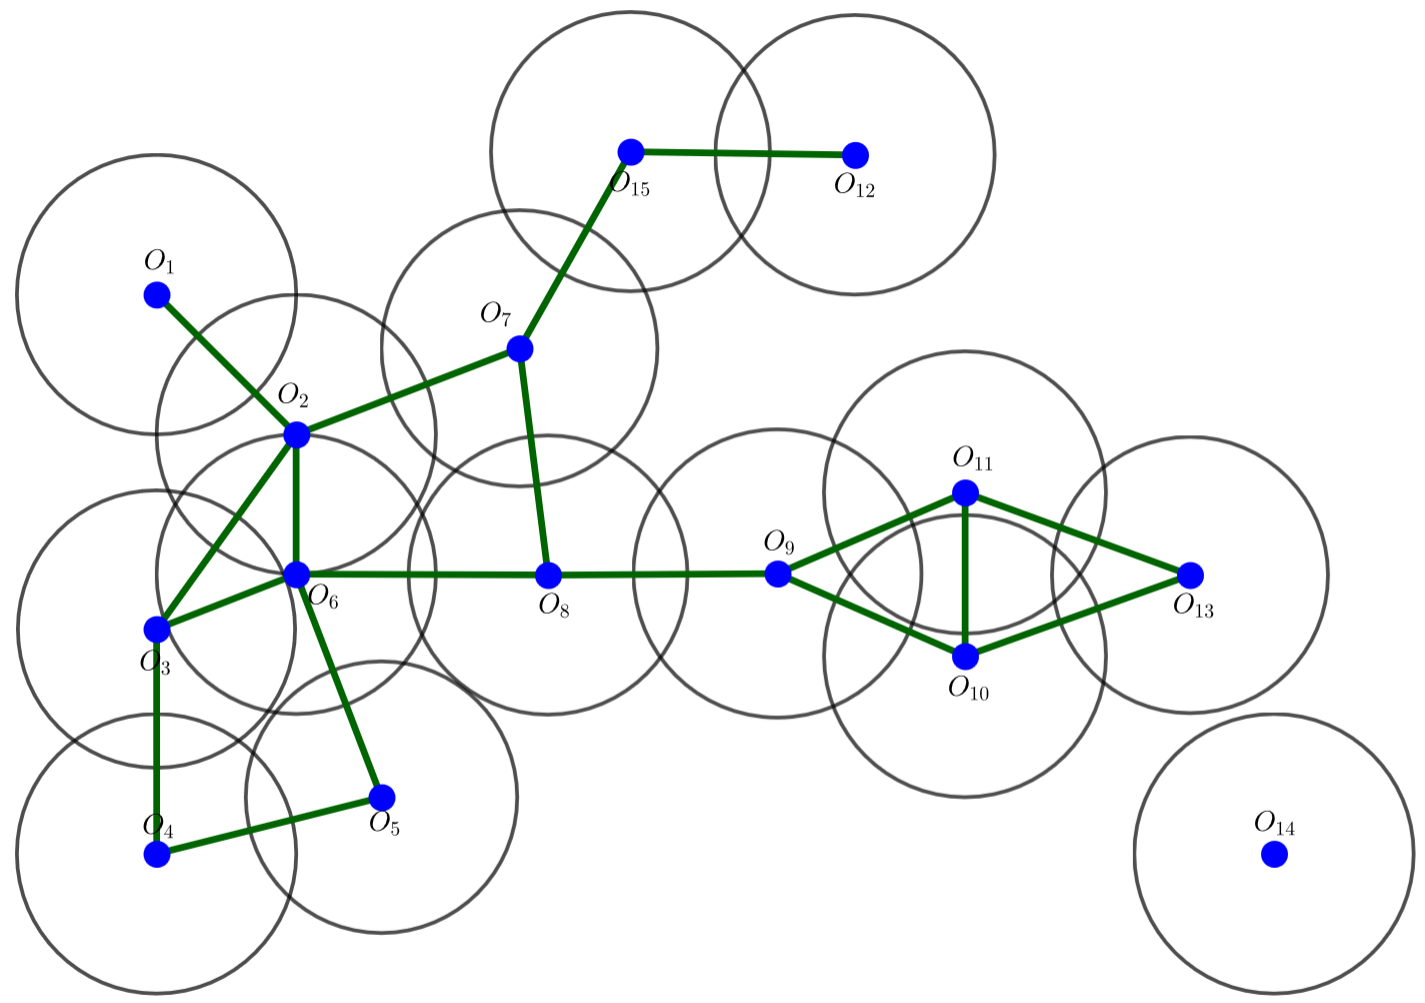
\includegraphics[width=0.8\textwidth]{./Images/02.png}
  \end{figure}
\end{frame}

\begin{frame}{...}
  Observemos su gráfica dual
  \begin{figure}  
    \centering
    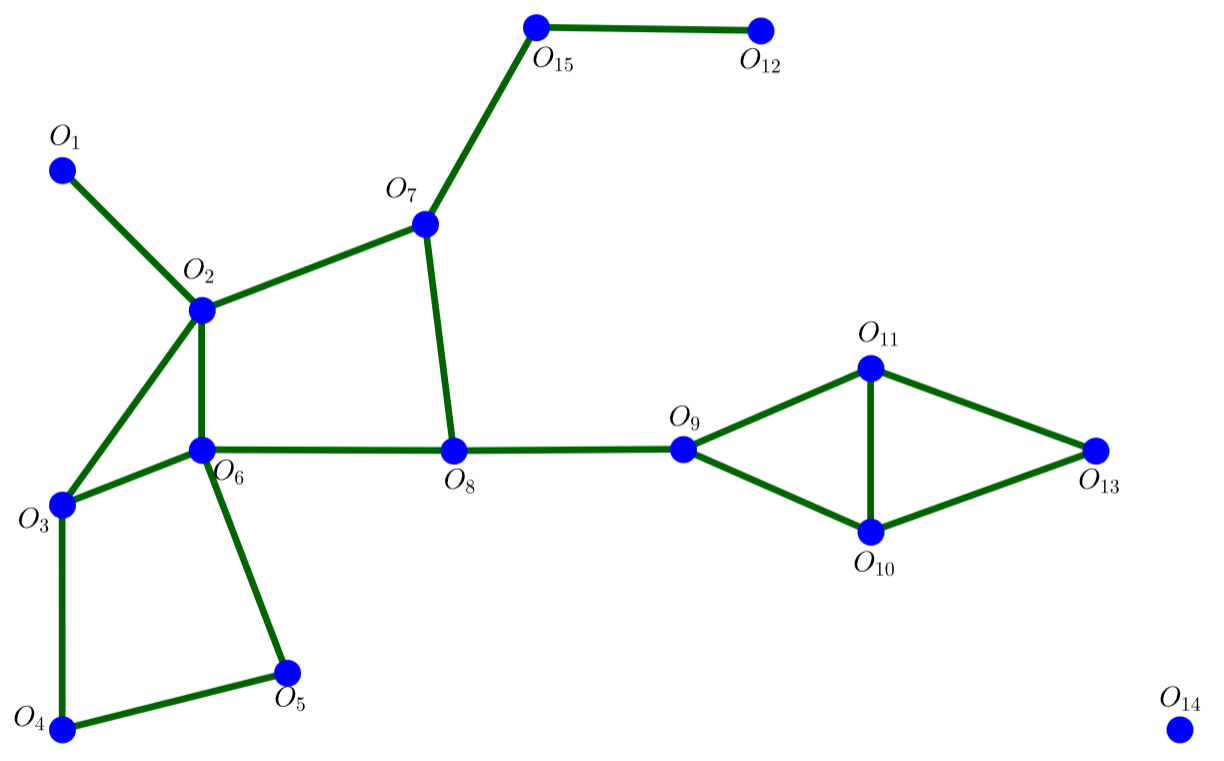
\includegraphics[width=0.8\textwidth]{./Images/SET.png}
  \end{figure}
  \textbf{Obs.} Existe un preprocesamiento que se encarga de exhibir candidatos a OPT.
\end{frame}

\begin{frame}{...}
  Sea $S_1 = \{O_1, O_6, O_4, O_7, O_{12}, O_9, O_{13}, O_{14}\}$
  \begin{figure}  
    \centering
    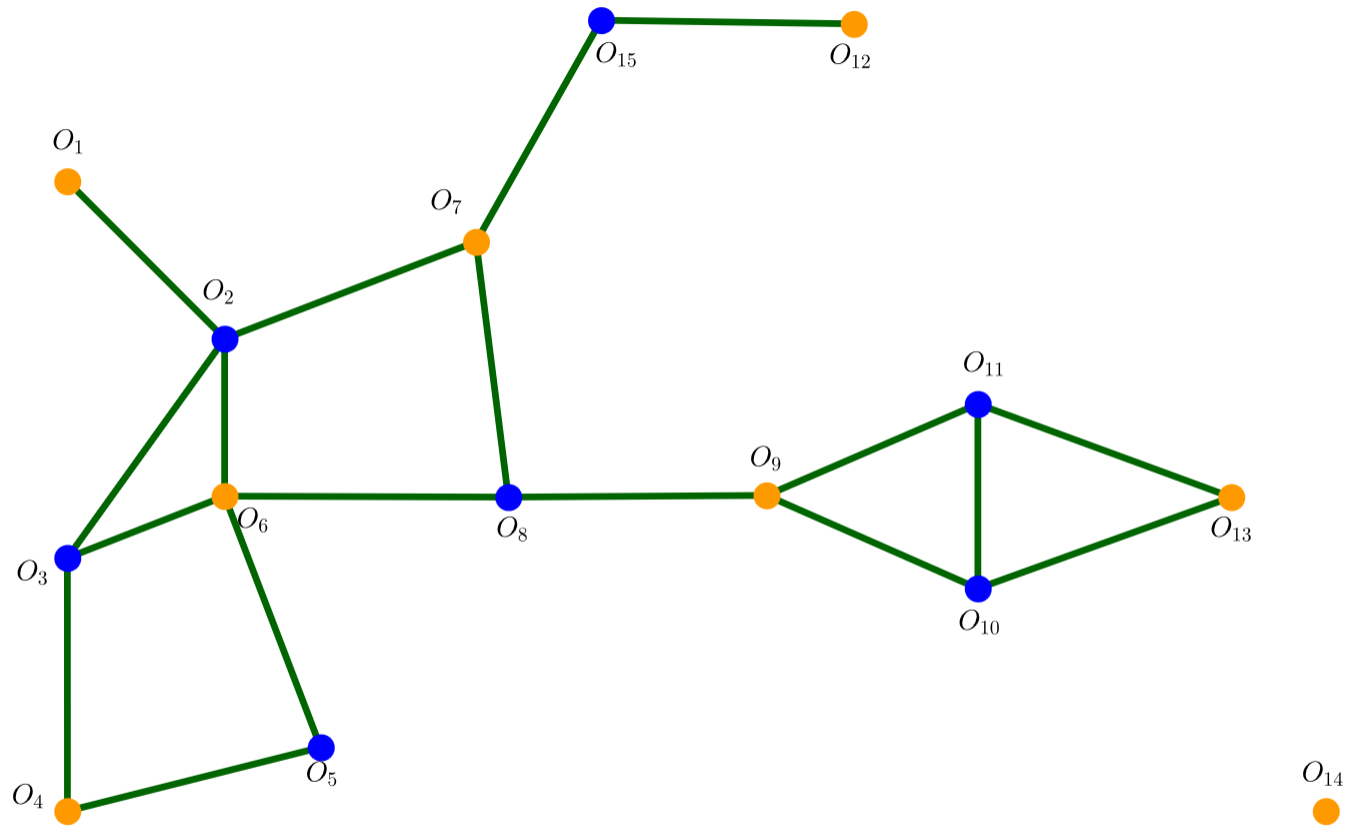
\includegraphics[width=0.8\textwidth]{./Images/S1.png}
  \end{figure}
\end{frame}

\begin{frame}{...}
  Sea $S_2 = \{O_2, O_4, O_8, O_{15}, O_{11}, O_{14}\}$
  \begin{figure}  
    \centering
    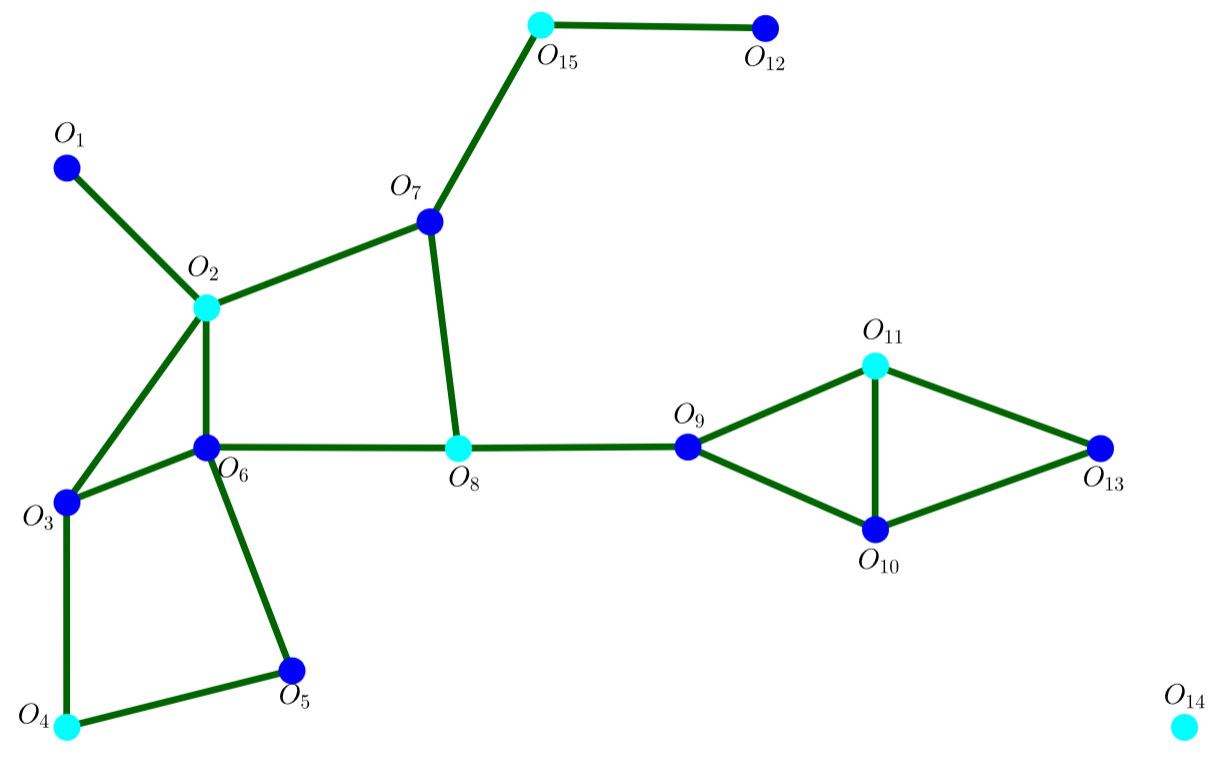
\includegraphics[width=0.8\textwidth]{./Images/S2.png}
  \end{figure}
\end{frame}


\begin{frame}{...}
  Sea $S_3 = \{O_1, O_3, O_5, O_7, O_{12}, O_{9}, O_{13}, O_{14}\}$
  \begin{figure}  
    \centering
    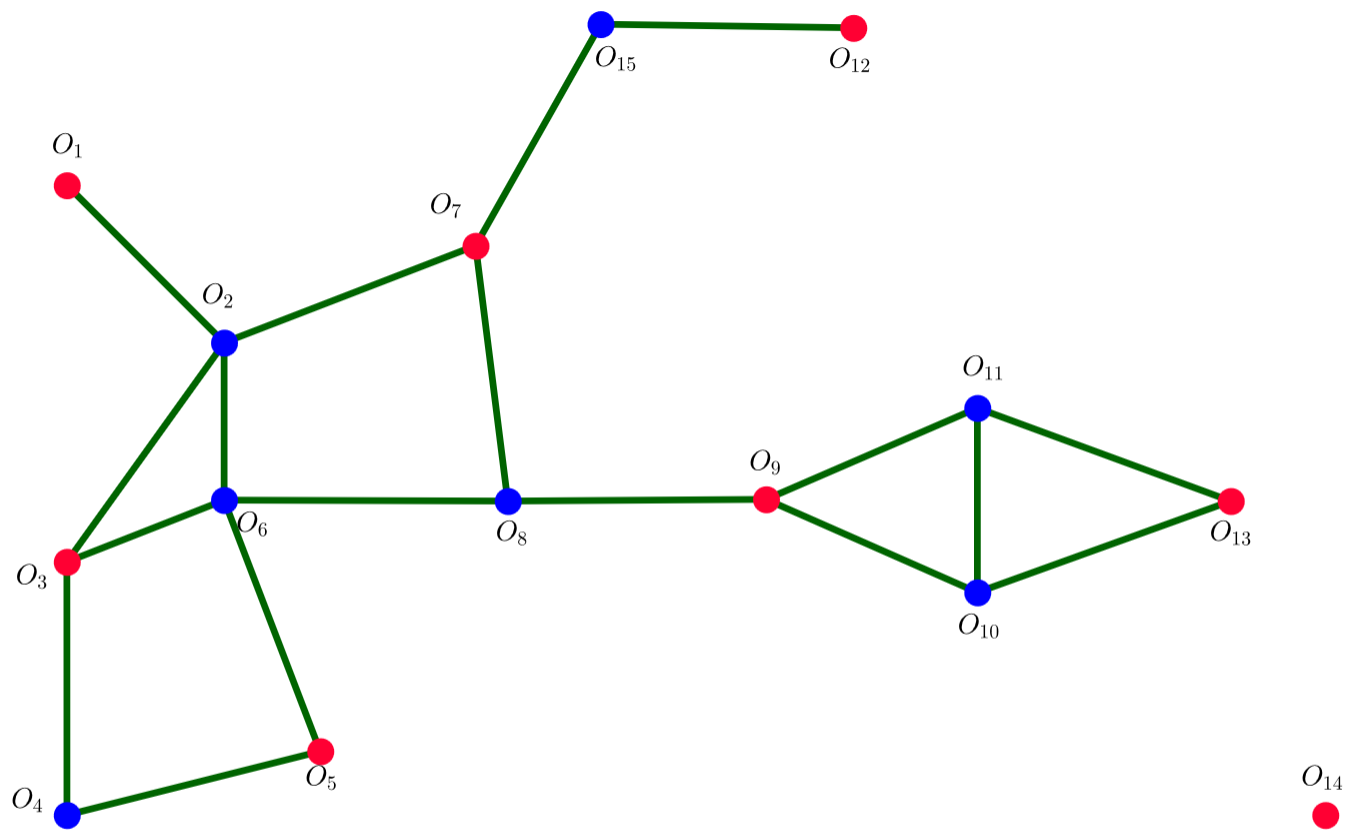
\includegraphics[width=0.8\textwidth]{./Images/S3.png}
  \end{figure}
\end{frame}

\begin{frame}{...}
  Sea $S_{MIS} = \{S_1, S_2, S_3\}$. Elijamos un candidato de $S_{MIS}$ tal que sea de mayor tamaño,
  digamos $S = S_1$. Ahora, eliminemos $O_{13}$.
  \begin{figure}  
    \centering
    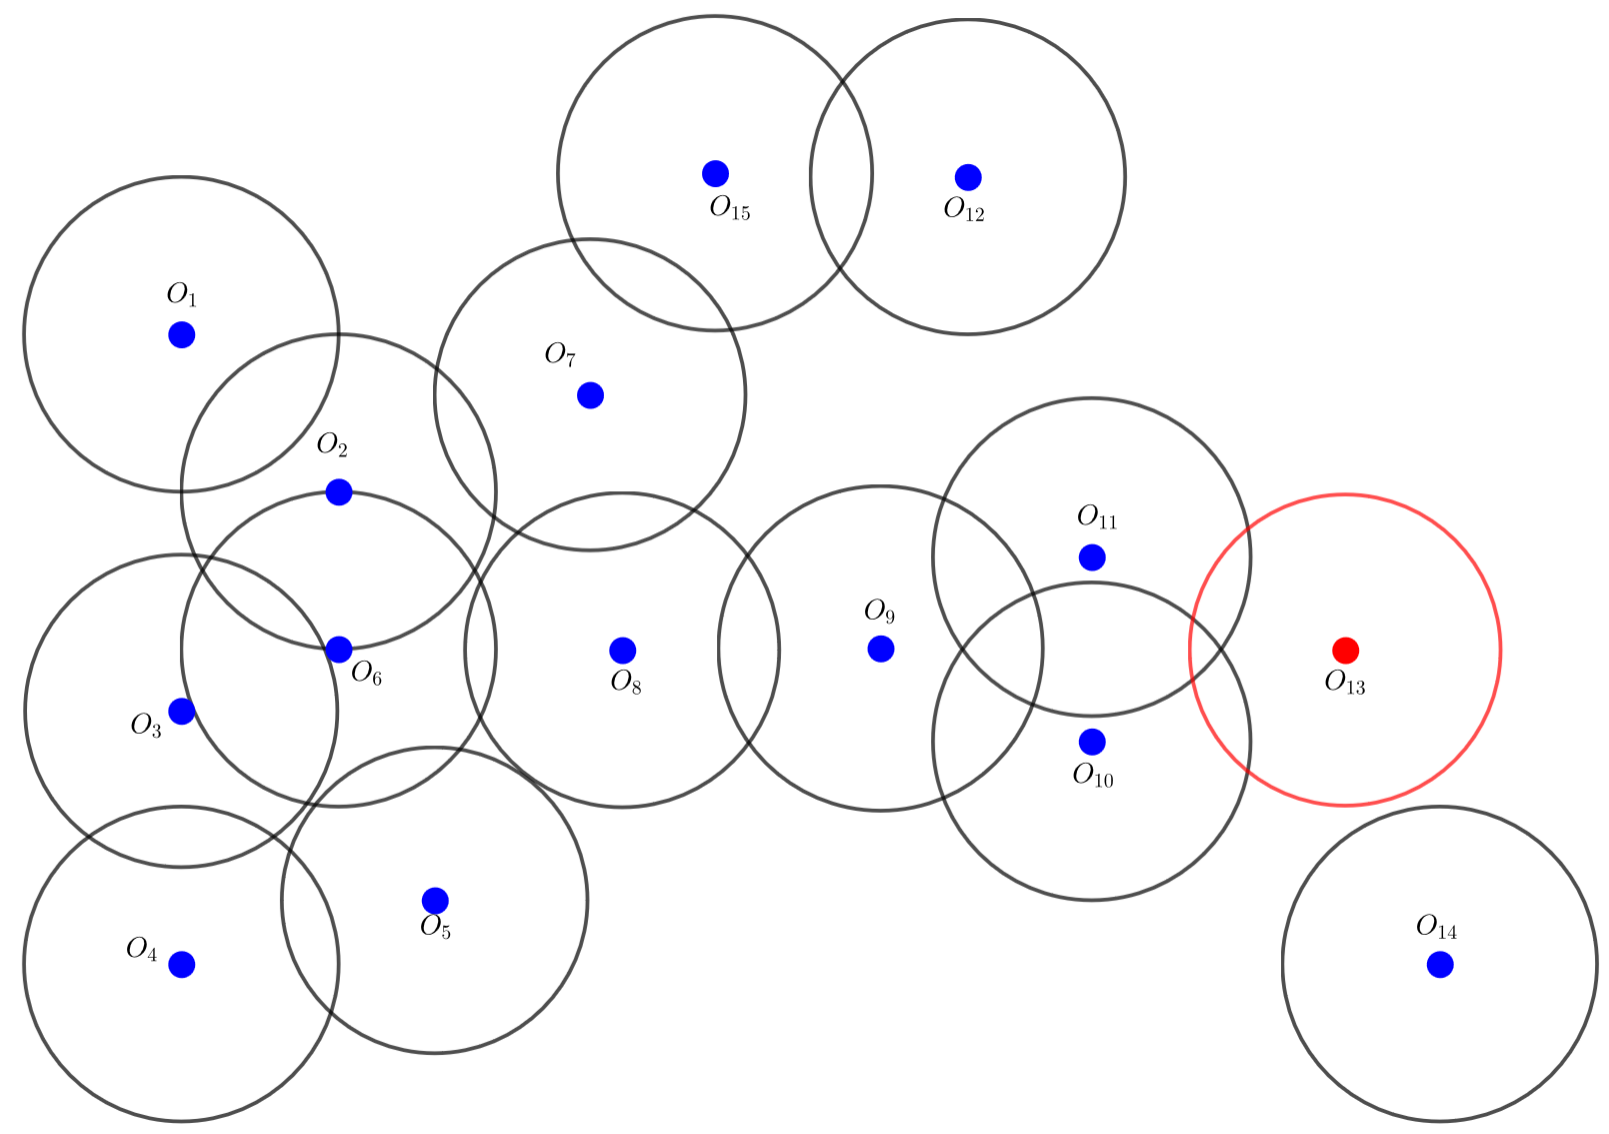
\includegraphics[width=0.8\textwidth]{./Images/03.png}
  \end{figure}
\end{frame}

\begin{frame}{...}
  Cómo hemos hecho una eliminación, debemos actualizar $S_1 = S_1/O_{13}$,
  $S_2 = S_2/O_{13}$, $S_3 = S_3/O_{13}$.
  \begin{figure}  
    \centering
    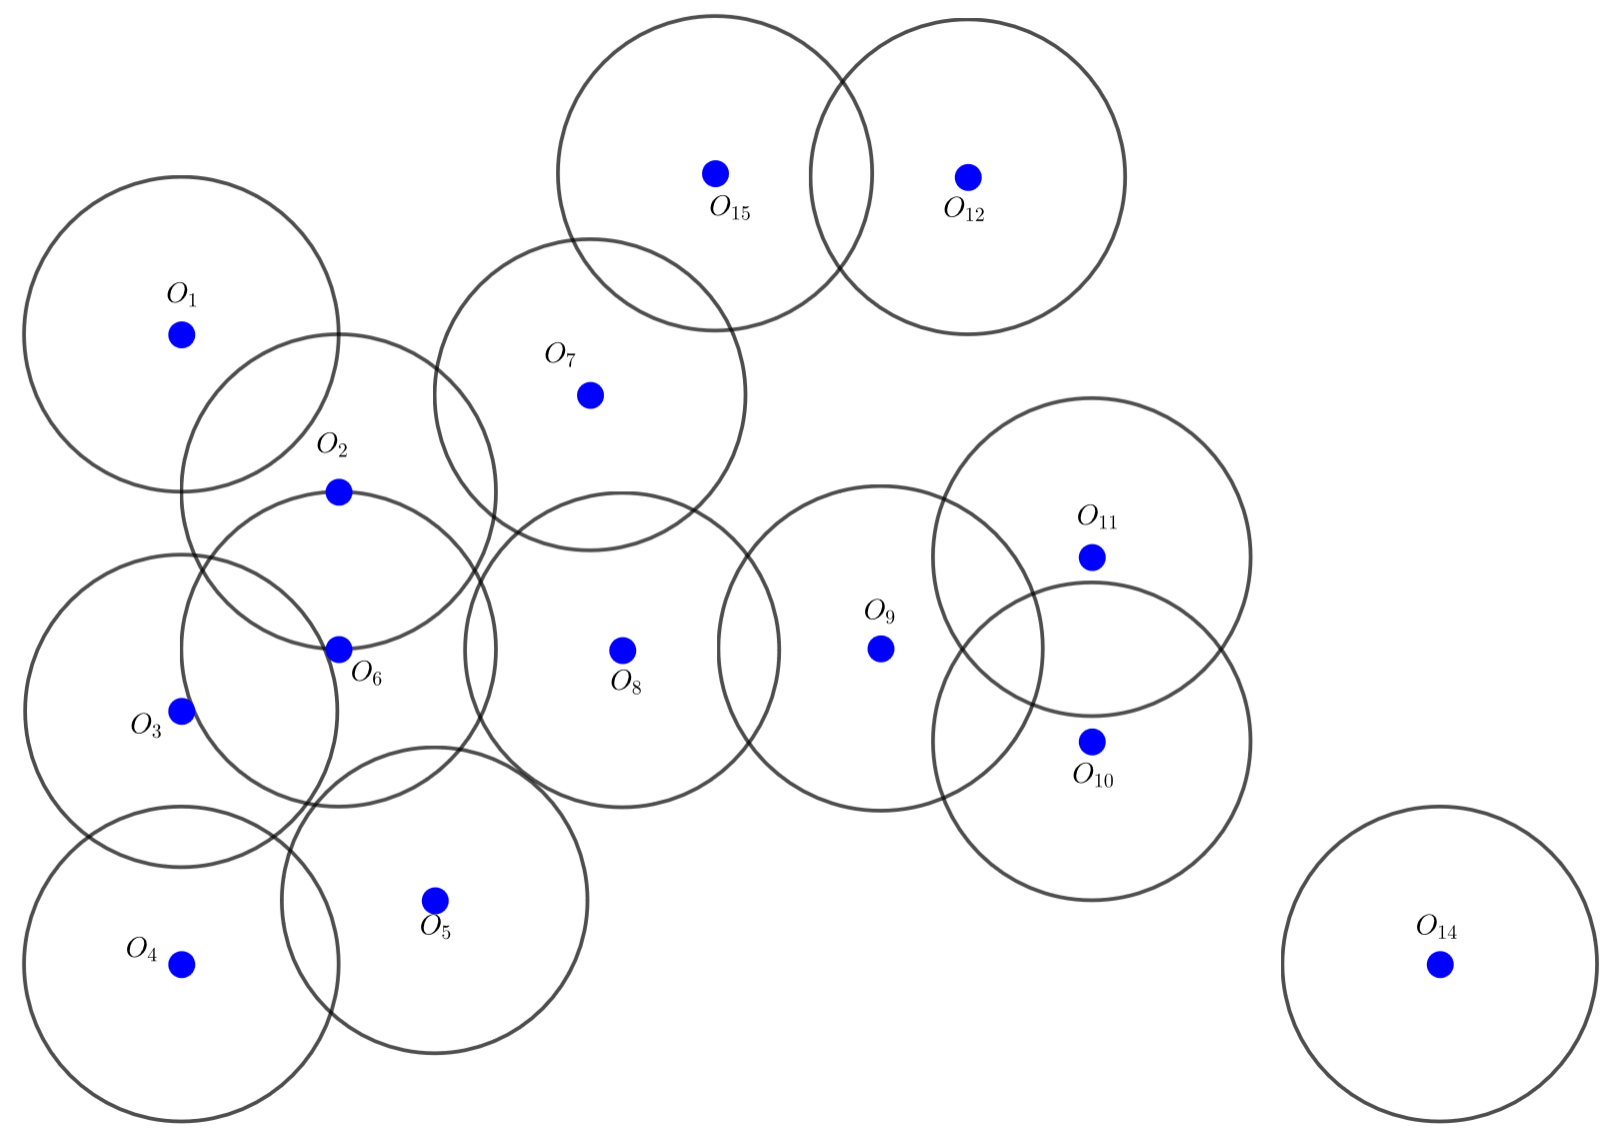
\includegraphics[width=0.8\textwidth]{./Images/04.png}
  \end{figure}
  $S = \{O_1, O_6, O_4, O_7, O_{12}, O_9, O_{14}\}$.
\end{frame}

\begin{frame}{...}
  Añadamos $O_{13}$ (un nuevo disco)
  \begin{figure}  
    \centering
    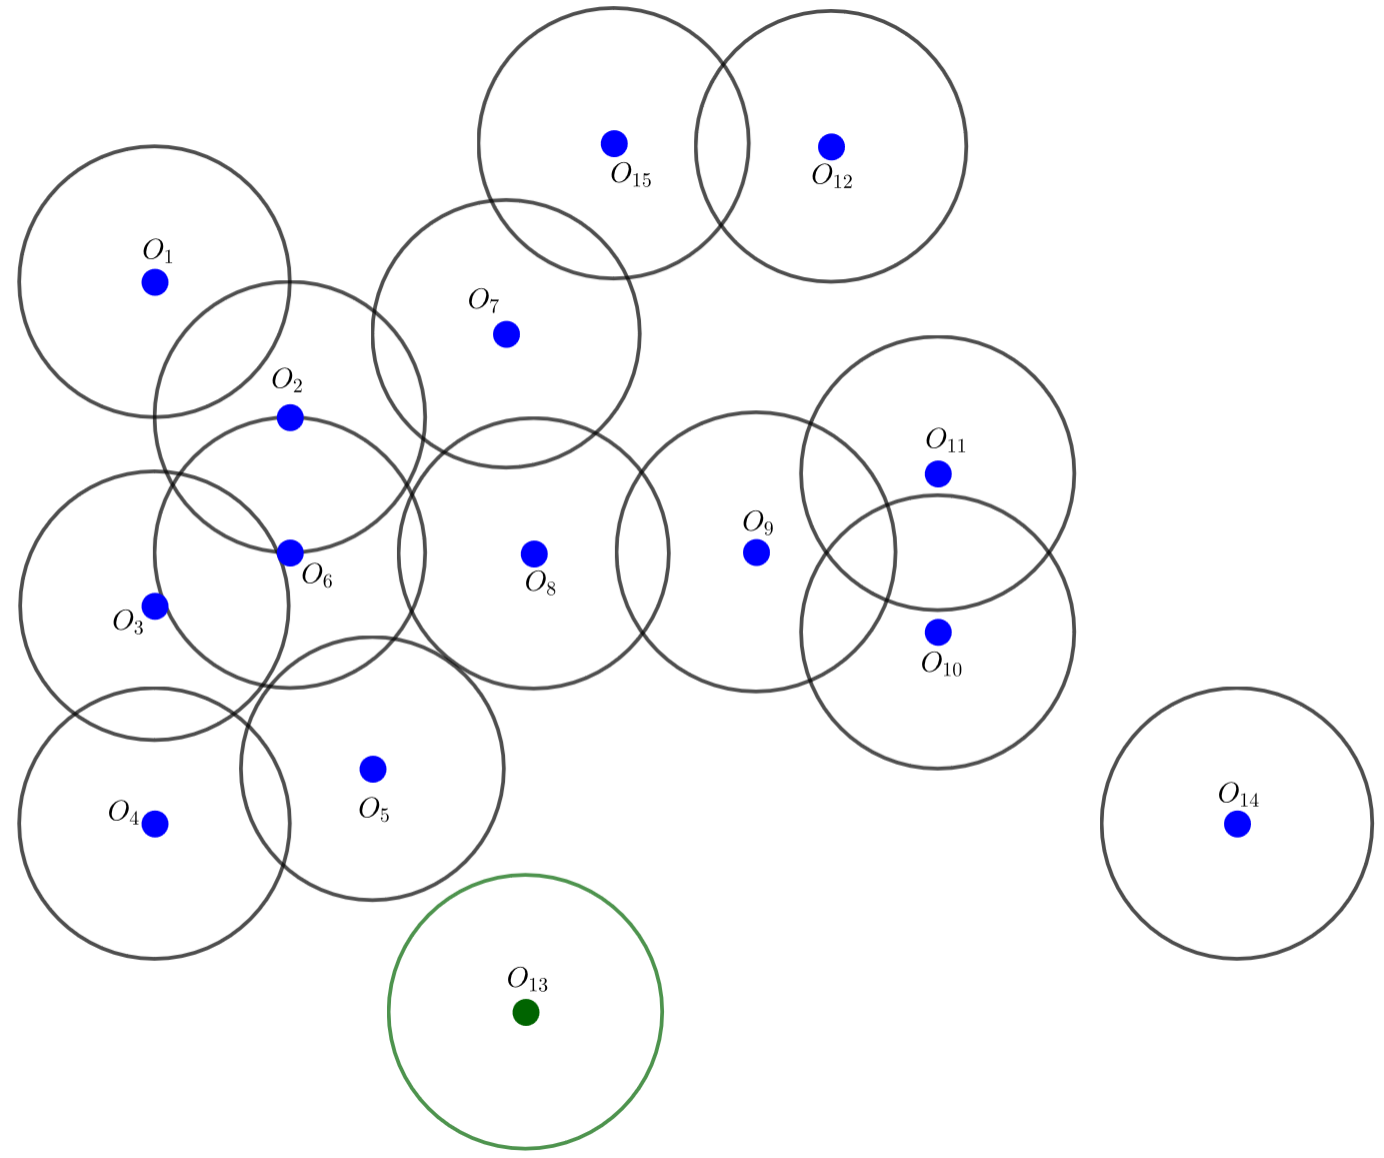
\includegraphics[width=0.7\textwidth]{./Images/05.png}
  \end{figure}

\end{frame}

\begin{frame}{...}
  Verificamos si este disco debe formar parte de los candidatos,
  en este caso actualizamos $S_1 = S_1 \cup \{O_{13}\}$, $S_2 = S_2 \cup \{O_{13}\}$,
  $S_3 = S_3 \cup \{O_{13}\}$. Y  $S = \{O_1, O_6, O_4, O_7, O_{12}, O_{13}, O_9, O_{14}\}$.
  \begin{figure}  
    \centering
    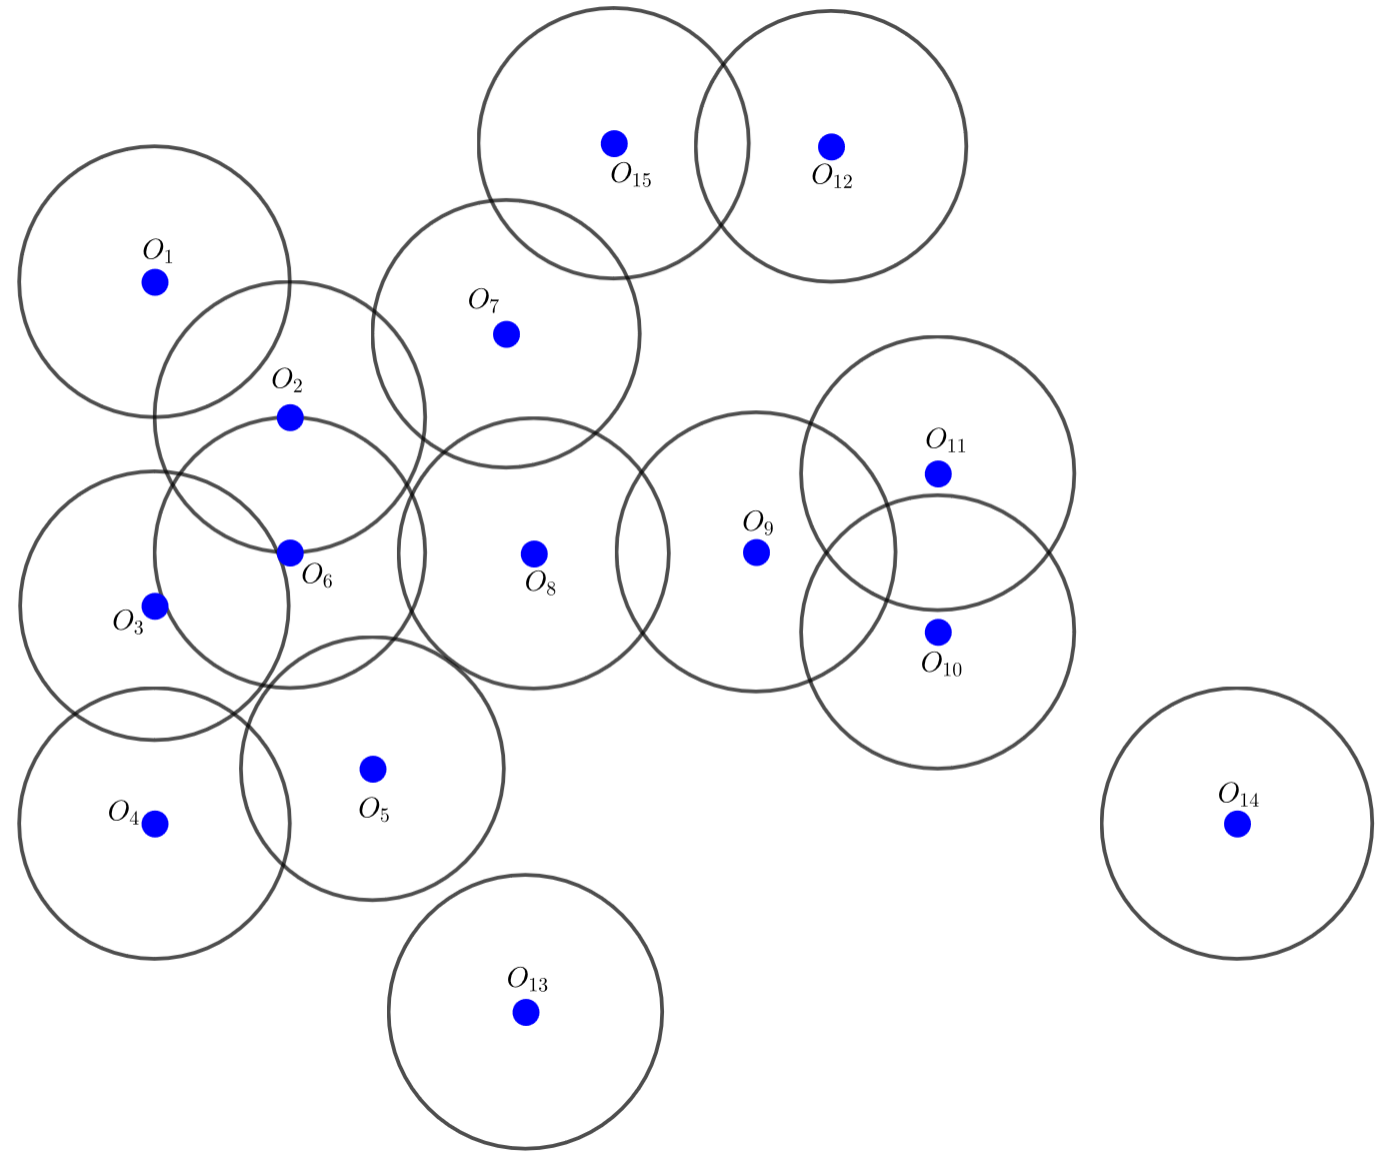
\includegraphics[width=0.7\textwidth]{./Images/06.png}
  \end{figure}
\end{frame}

\begin{frame}{...}
  Eliminemos $O_{15}$
  \begin{figure}  
    \centering
    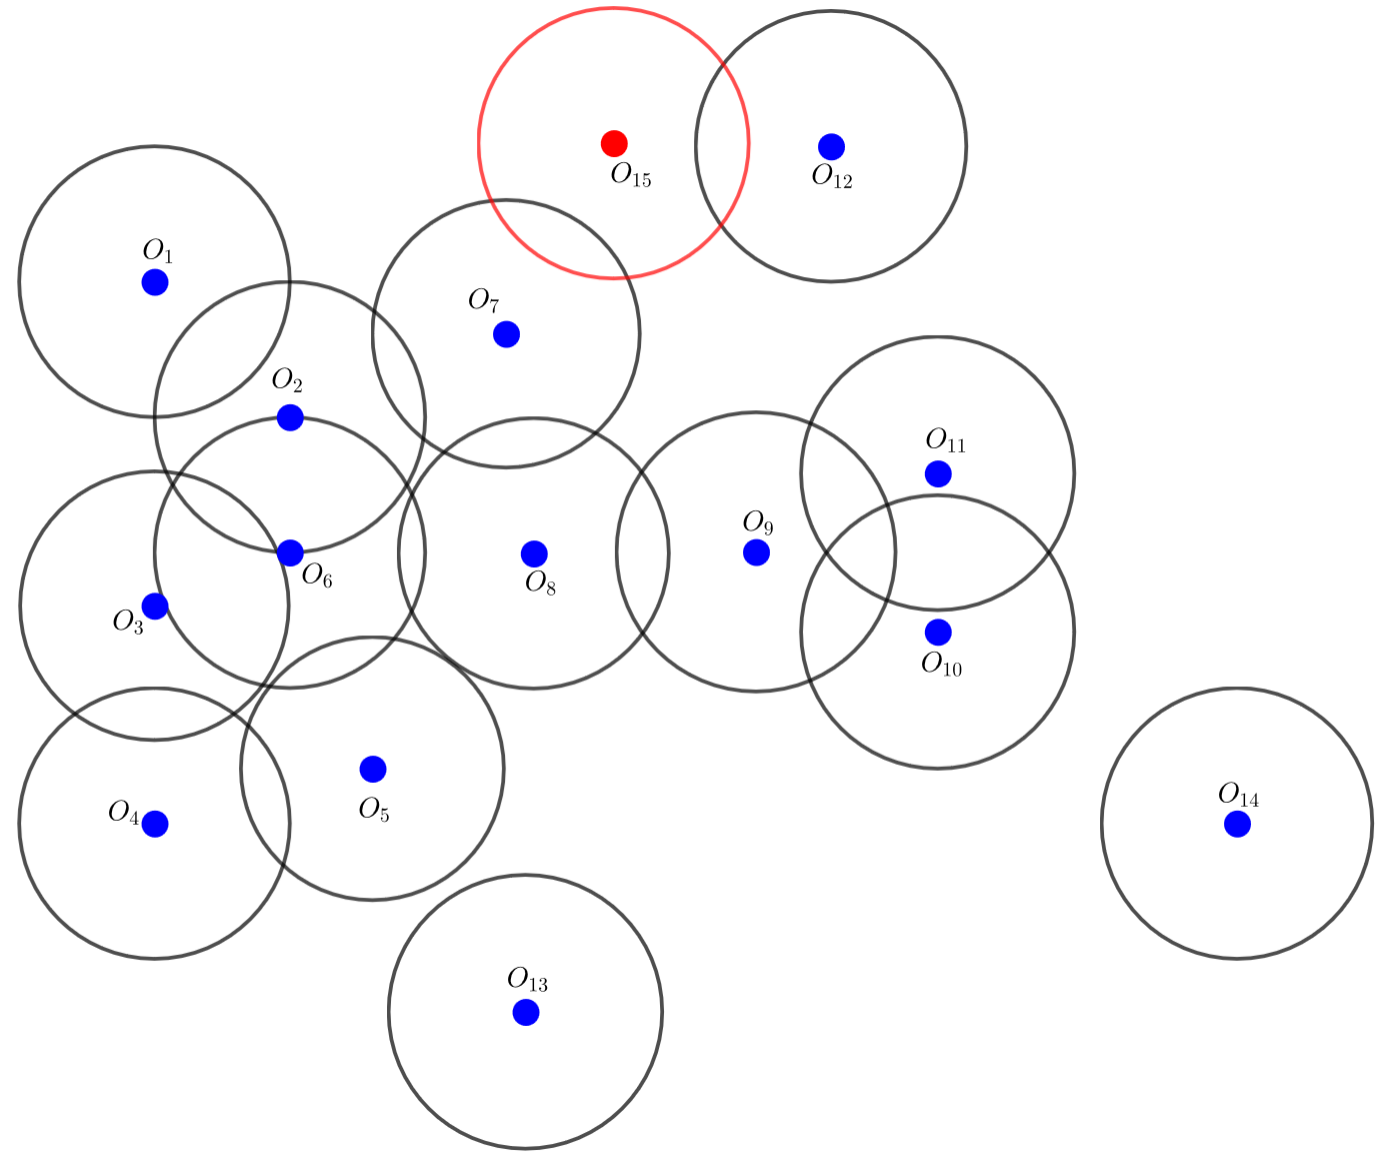
\includegraphics[width=0.7\textwidth]{./Images/07.png}
  \end{figure}
\end{frame}

\begin{frame}{...}
  Verificamos si está eliminación afecta a nuestros candidatos, en este caso
  no se ven afectados y continuamos
  \begin{figure}  
    \centering
    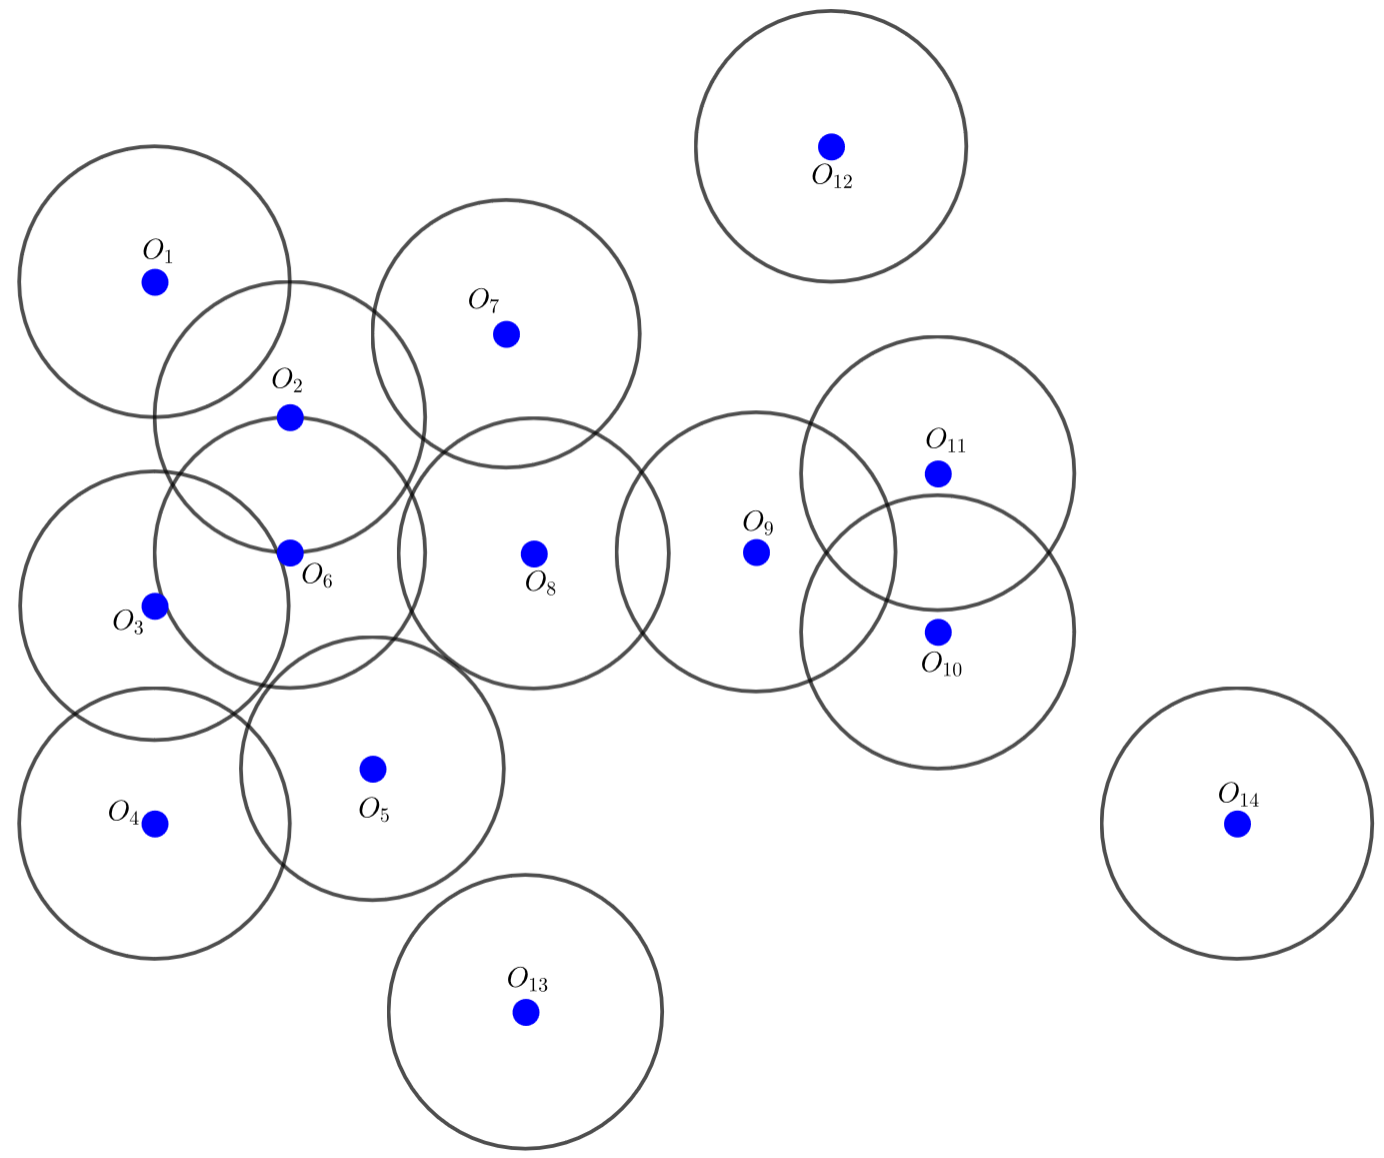
\includegraphics[width=0.7\textwidth]{./Images/08.png}
  \end{figure}
  $S = \{O_1, O_6, O_4, O_7, O_{12}, O_{13}, O_9, O_{14}\}$
\end{frame}

\begin{frame}{...}
  Eliminamos $O_{14}$
  \begin{figure}  
    \centering
    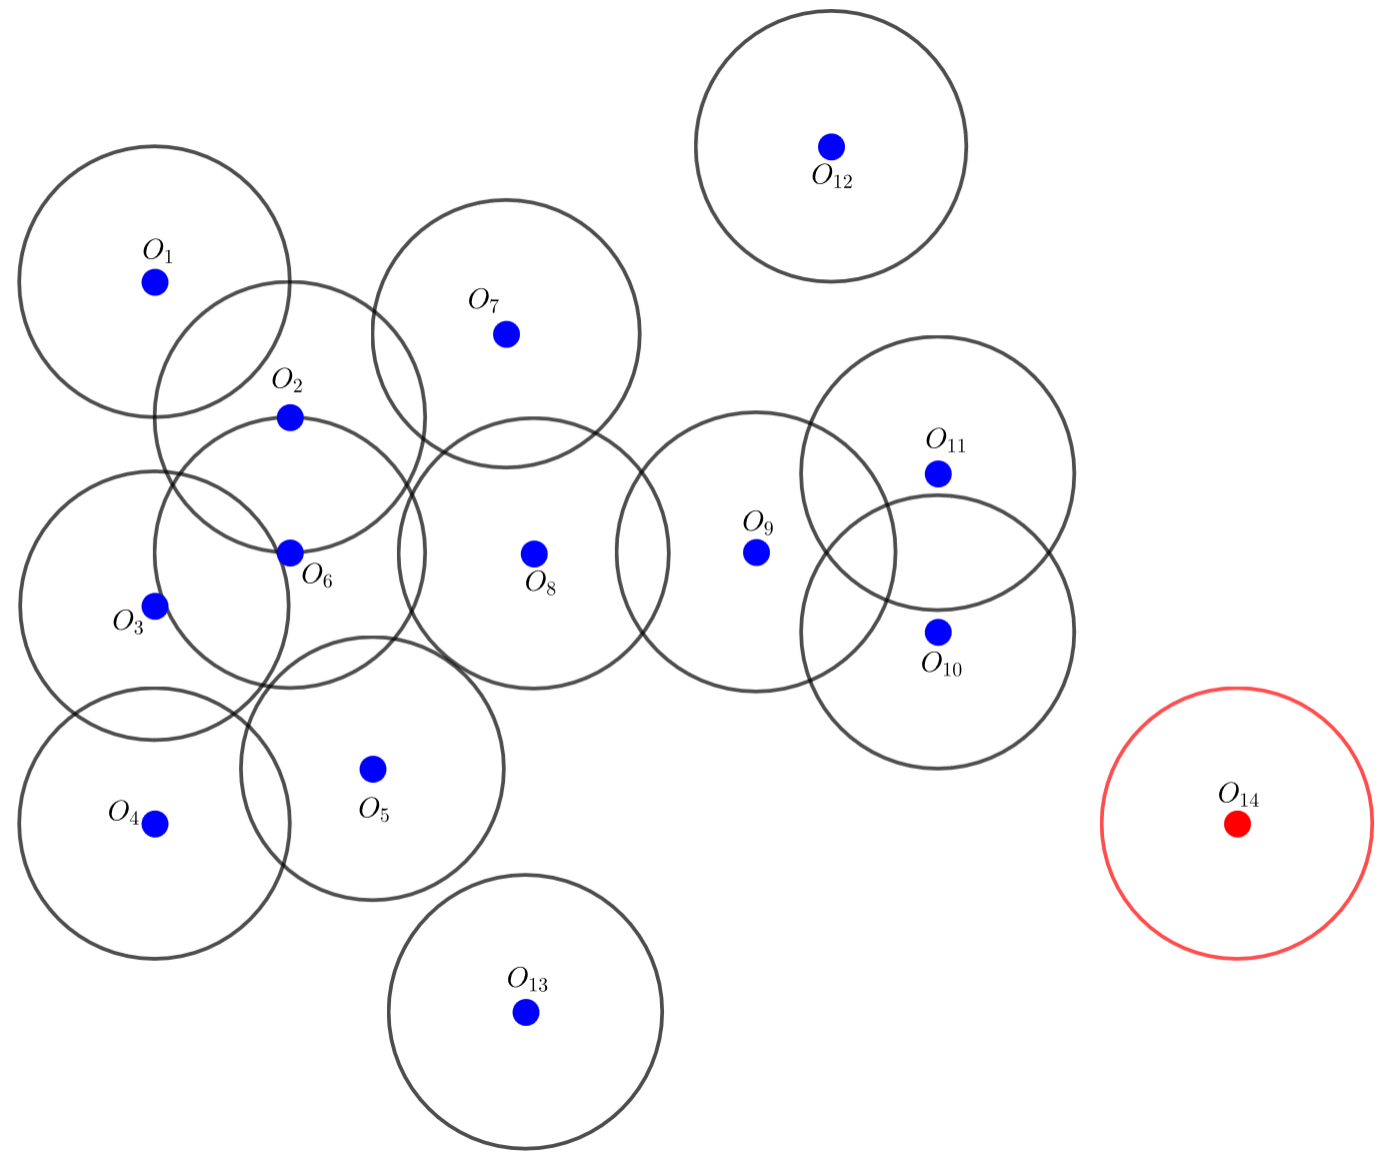
\includegraphics[width=0.7\textwidth]{./Images/09.png}
  \end{figure}
  
\end{frame}

\begin{frame}{...}
  Actualizamos los estados de nuestros candidatos $S_1 = S_1/O_{14}$,
  $S_2 = S_2/O_{14}$, $S_3 = S_3/O_{14}$.
  \begin{figure}  
    \centering
    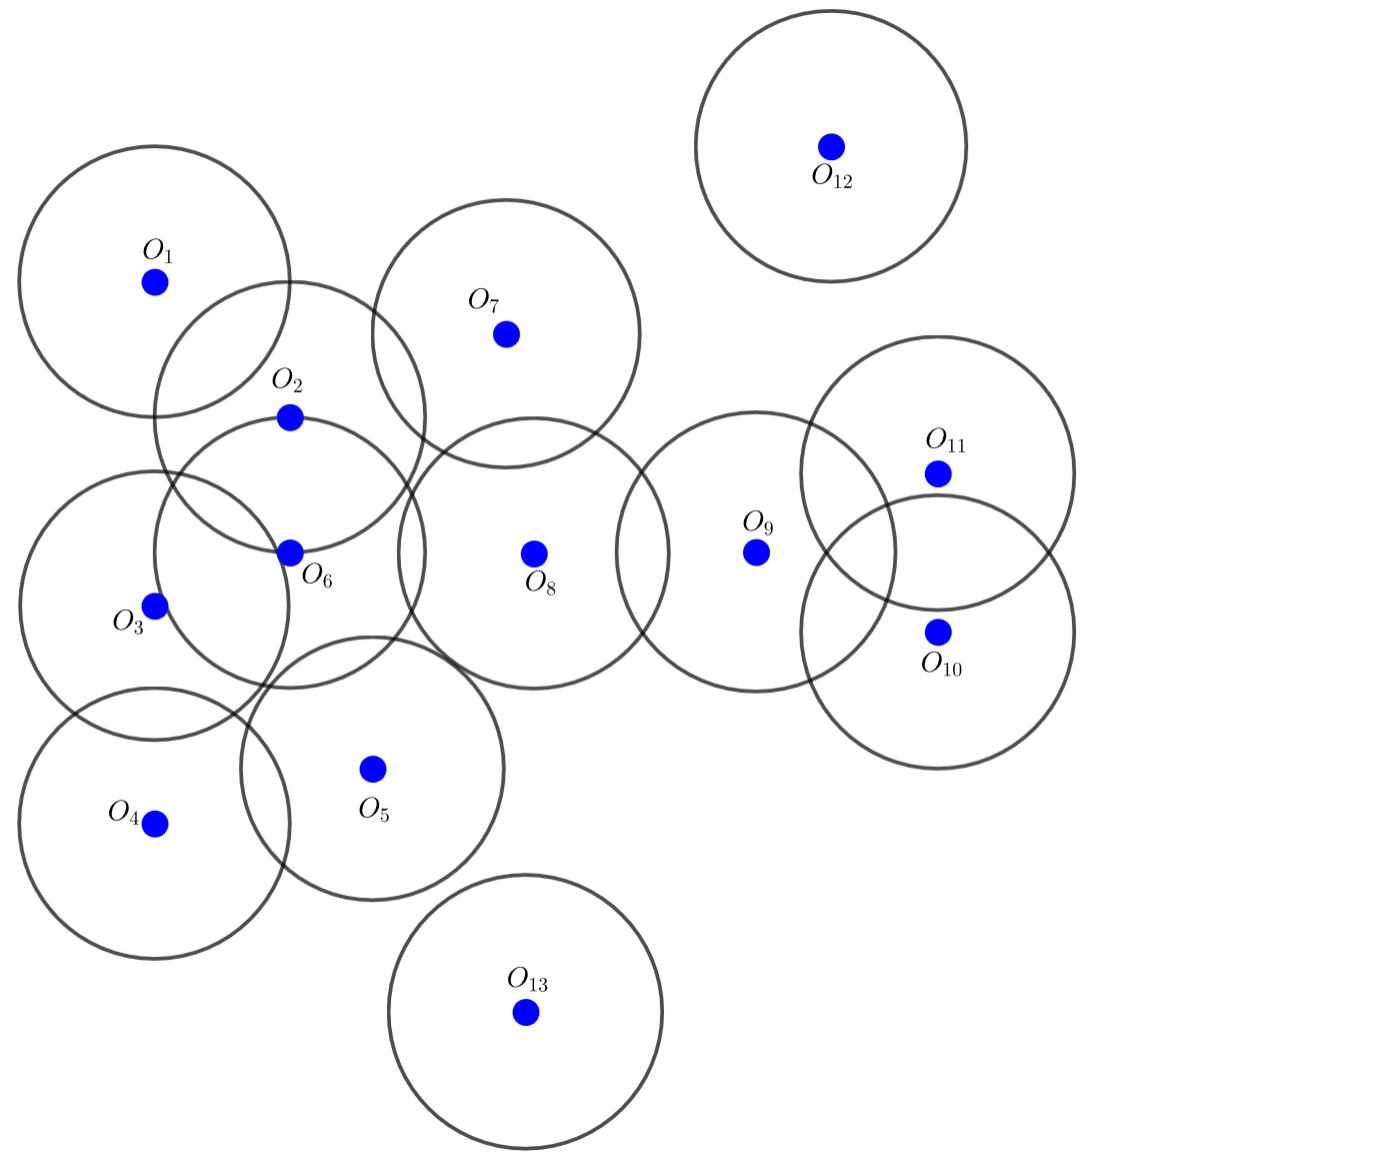
\includegraphics[width=0.7\textwidth]{./Images/10.png}
  \end{figure}
    $S = \{O_1, O_6, O_4, O_7, O_{12}, O_{13}, O_9\}$. \textbf{FIN.}
\end{frame}

\subsection{Restricciones de uso.}
\begin{frame}{Restricciones}
  Restricciones:
  \begin{itemize}[<+->]
  \item La función de transición suave MIX sólo funciona en objetos
    geométricos $f$-fat con $f \in \mathbb{R}$ y $f>0$.
    \begin{figure}  
      \centering
      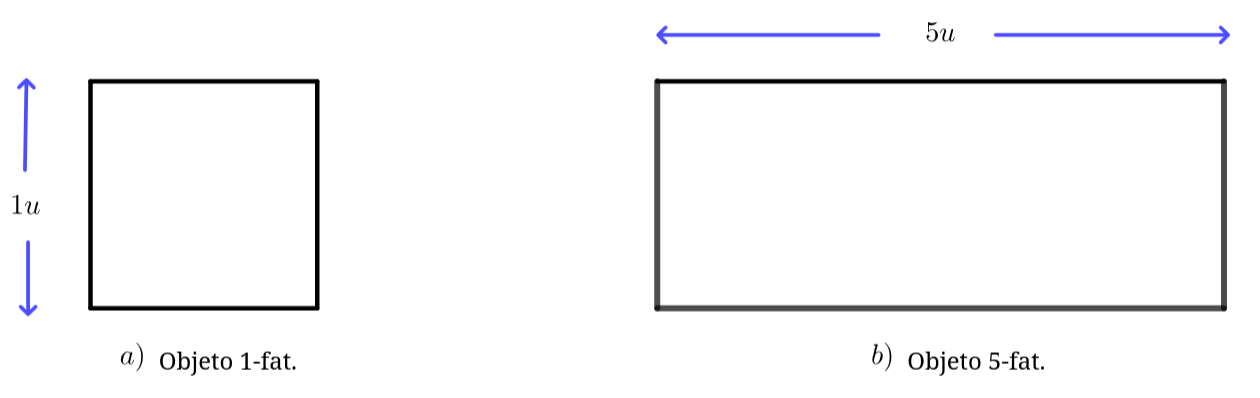
\includegraphics[width=0.7\textwidth]{./Images/fat.png}
    \end{figure}
  \item La función recibe dos estados $S_i, S_f$ y transita de $S_i$
    a $S_f$ en $\mathcal{O}(\alpha \log \alpha)$, pues debe ordenar
    cada conjunto de entrada.
  \item Sólo funciona para $\mathbb{R}^d$ con $d$ constante.
  \item Se pueden realizar, a lo más, $5u$ eliminaciones o adiciones,
    con $u \in \mathbb{Z}^+$, asumiendo $u > 0$.
  \item Las eliminaciones se realizan de manera directa, las adiciones
    se realizan al final de la ejecución del algoritmo. Basta guardar
    las adiciones en una cola.
  \item La cantidad de conjuntos candidatos es $K \in \mathcal{O}(1)$.
  \end{itemize}
\end{frame}

%\subsection{Análisis de tiempo.}
%----------------------------------------------
\mysection{Estructuras de datos empleadas}
\subsection{Vecino más cercano/lejano.}
\begin{frame}{Observaciones}
  Para un cuadrado $2 \times 2$, puede contener,
  a lo más, $4$ discos unitarios que no se intersecten
  \begin{figure}  
    \centering
    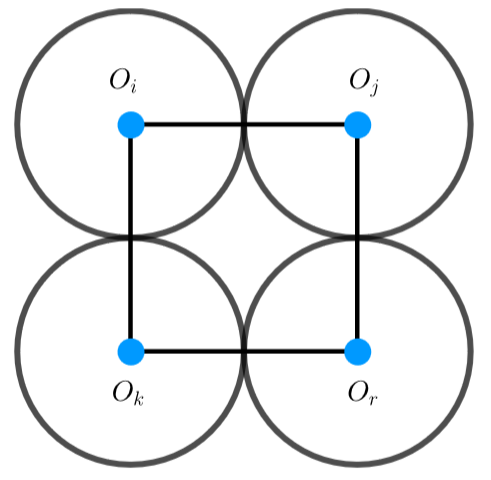
\includegraphics[width=0.4\textwidth]{./Images/4.png}
  \end{figure}
\end{frame}

\begin{frame}{Construcción de rejillas desplazadas}
 Construcción:
  \begin{itemize}[<+->]
  \item Definimos cuadrículas, por conjunto candidato, $G_1, \dotsm, G_k$. Estas pueden
    ser distintas y en ocasiones iguales
    \begin{figure}  
      \centering
      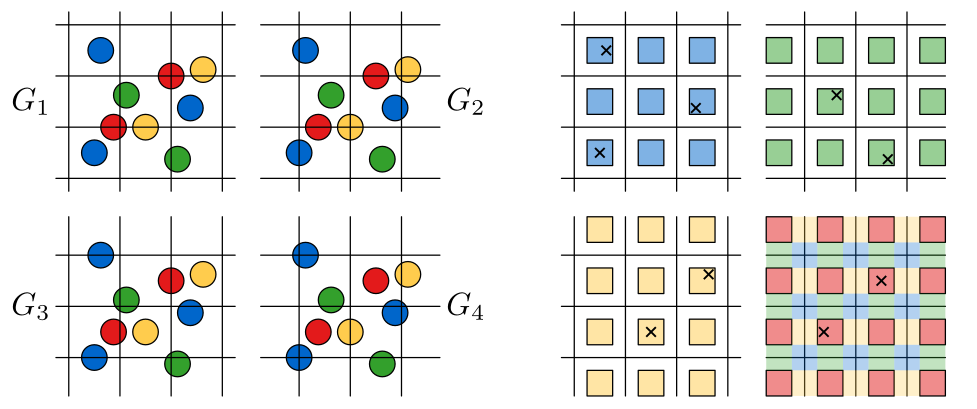
\includegraphics[width=0.4\textwidth]{./Images/cuadricula.png}
    \end{figure}
  \item Cada celda puede ser definida de longitud $4$ o trabajar celdas de
    longitud 2 de manera unificada.
  \item Para $G_1$ tenemos las líneas $\{x = 4i\}$ y $\{y = 4i\}$ con
    $i \in \mathbb{Z}^+$. Análogo para longitud 2.
  \item Para las siguientes $G_2$ y $G_3$ marcamos $\{x = 4i + 2\}$ y $\{y = 4i + 2\}$
    respectivamente.
  \item $G_4$ se deplaza en ambos sentidos $\{x = 4i + 2\}$ y $\{y = 4i + 2\}$. Esto se
    sigue de manera iterativa.
  \item La celda cumple la propiedad de consultar por intersecciones de discos más cercanos
    y enocntrar el disco más lejano dado un disco. La última propiedad no la utilizaremos en
    nuestro caso.
  \end{itemize}
\end{frame}

\begin{frame}
  En nuestro caso, usemos la reja de tamaño $2$, con la concideración de que cada
  centro de disco se encuentra en una única celda. Así, para $S_1$ tenemos que
  \begin{figure}  
    \centering
    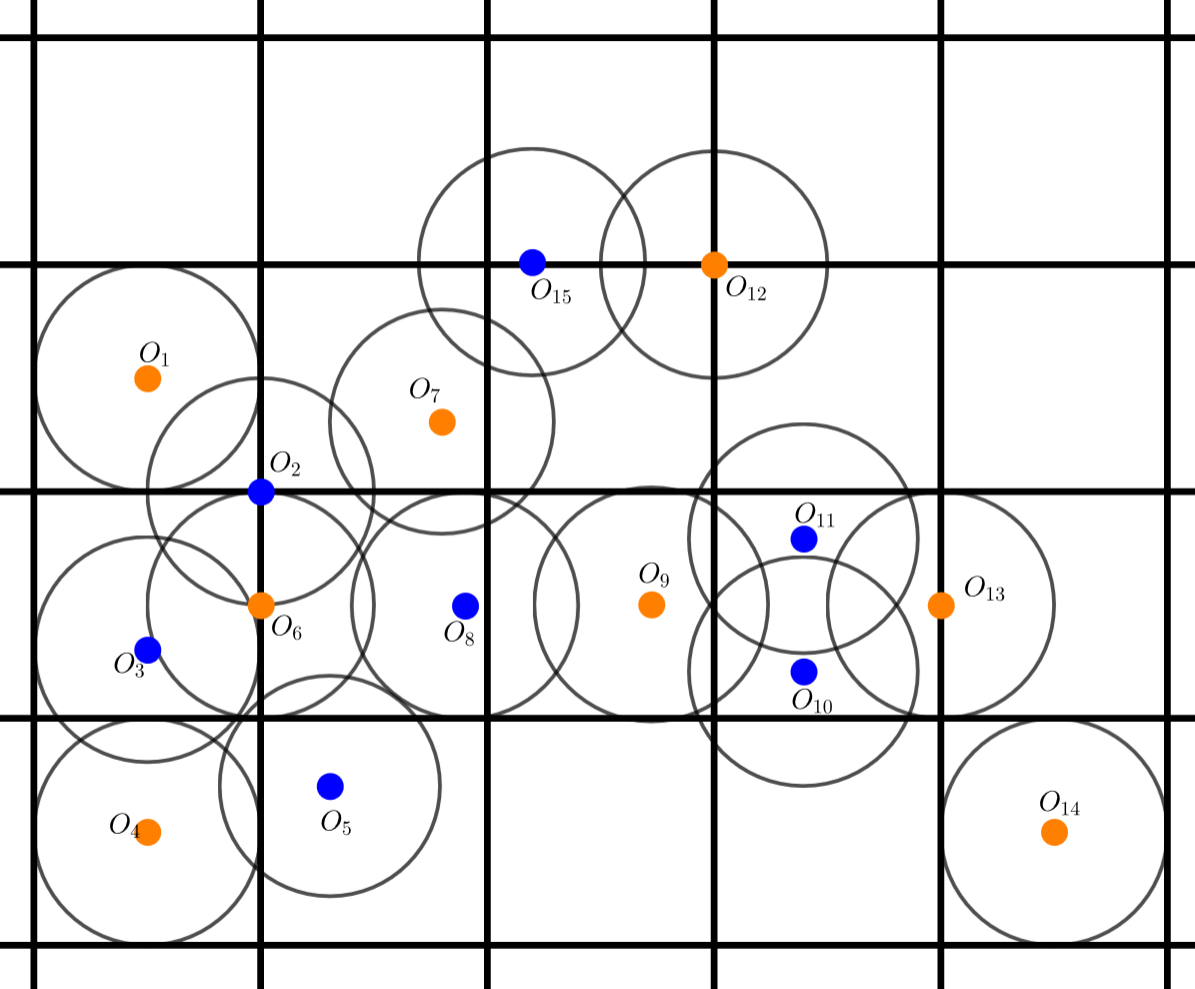
\includegraphics[width=0.7\textwidth]{./Images/R1.png}
  \end{figure}
\end{frame}

\begin{frame}
  Para $S_2$ tenemos que
  \begin{figure}  
    \centering
    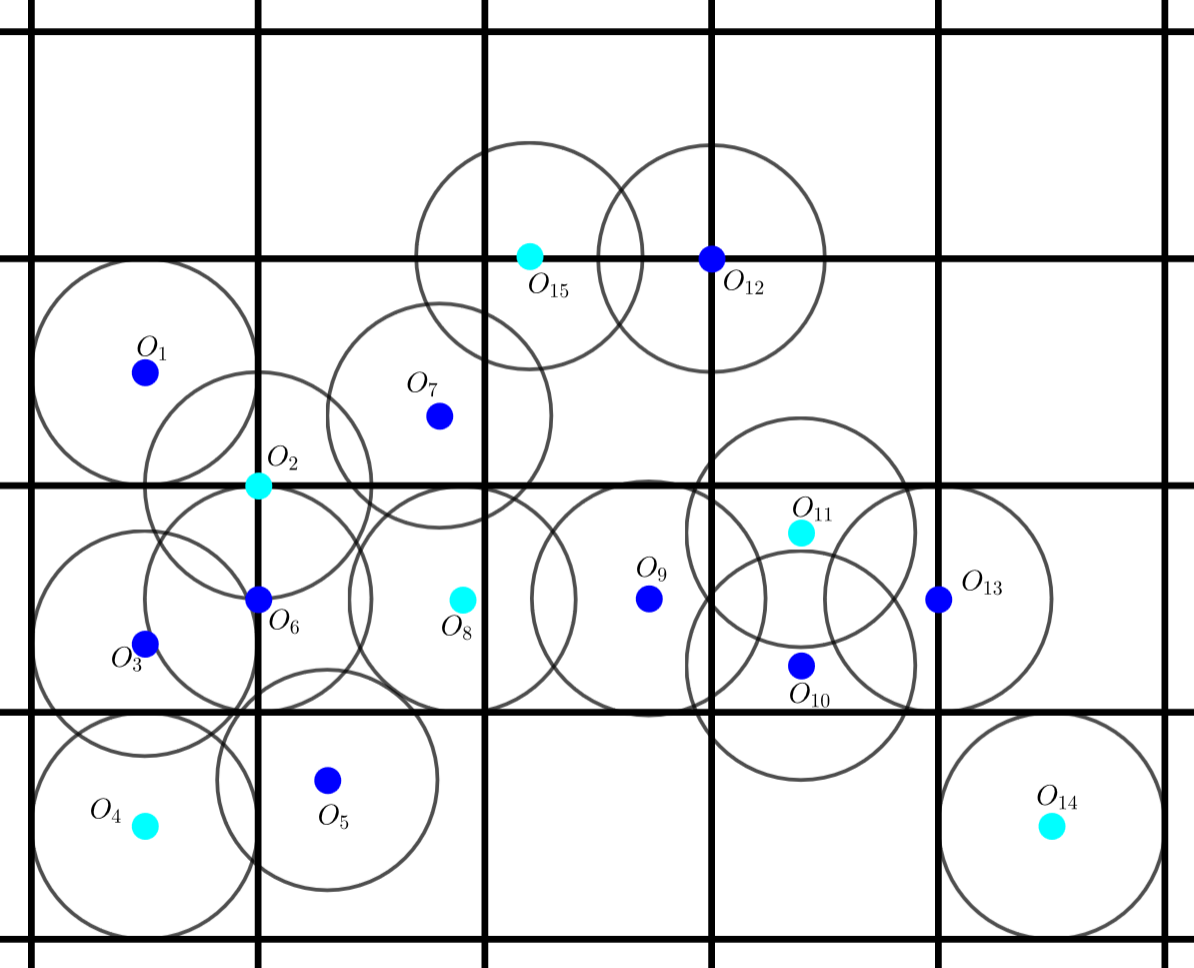
\includegraphics[width=0.7\textwidth]{./Images/R2.png}
  \end{figure}
\end{frame}

\begin{frame}
  Para $S_3$ tenemos que
  \begin{figure}  
    \centering
    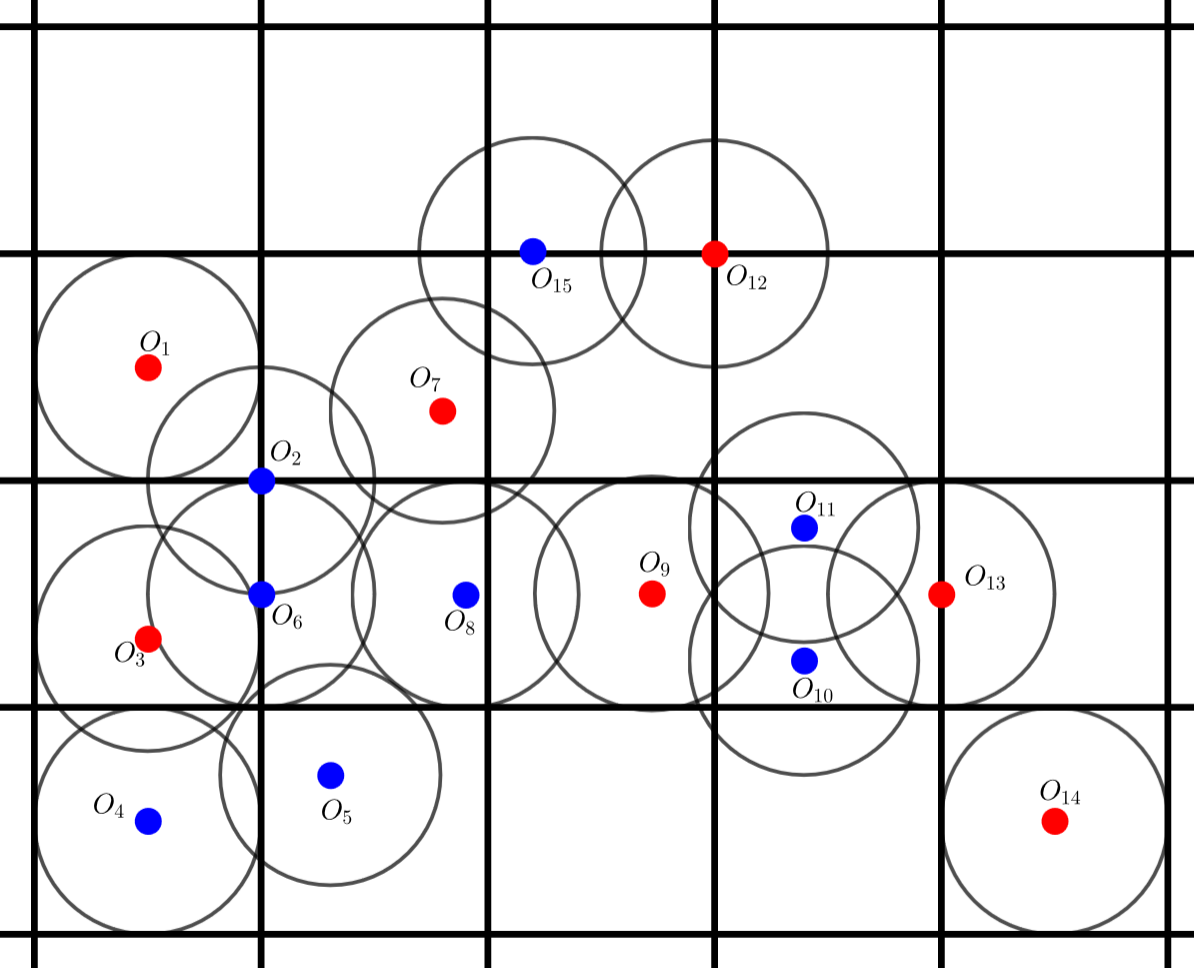
\includegraphics[width=0.7\textwidth]{./Images/R3.png}
  \end{figure}
\end{frame}

\begin{frame}
  \begin{block}{Lema 1.}
    Cada disco unitario en $\mathbb{R}^2$ está contenido en una celda de, al menos, una de las
    cuadrículas desplazadas $G_1, \dotsm, G_k$. En consecuencia para un conjunto $S$ de discos
    unitarios la celda de una de las rejillas contiene conjuntamente
    \[\frac{|S|}{4}\]
    discos.
  \end{block}
  \textbf{Dem.} La primera parte se da a partir de su construcción. La segunda parte se sigue
  del principio de casillas. \hfill $\square$\newline

  Gracias a este lema sabemos que una cuadrícula contiene al menos una fracción constante
  ($o(1)$) de la aproximación de OPT.
\end{frame}


\begin{frame}
  \begin{block}{Lema 2.}
    Sean $S_1, \dotsm S_k$ conjuntos independientes en el conjunto $D$ de discos unitarios
    calculados para $G_1, \dotsm G_k$ respectivamente. El más grande de $S_1, \dotsm,S_k$
    es una $12$-aproximación de MIS, para $D$.
  \end{block}
  \textbf{Dem.} Observar el caso en dónde $|S_i| = 1$ para rejillas $4 \times 4$ (este caso
  no es válido, pero da la idea de la prueba).\newline

  \textbf{Obs.} Una $x$-aproximación es una aproximación en $\frac{1}{x}$ que se puede
  interpretar cómo OPT - $x$, pero núnca cómo OPT + $x$.
\end{frame}

\subsection{Uso de un árbol conocido ...}
\begin{frame}{Resultado de MIX}
  $S$ ha sido el resultado de usar MIX, entonces nos retorna la siguiente gráfica

  \begin{figure}  
    \centering
    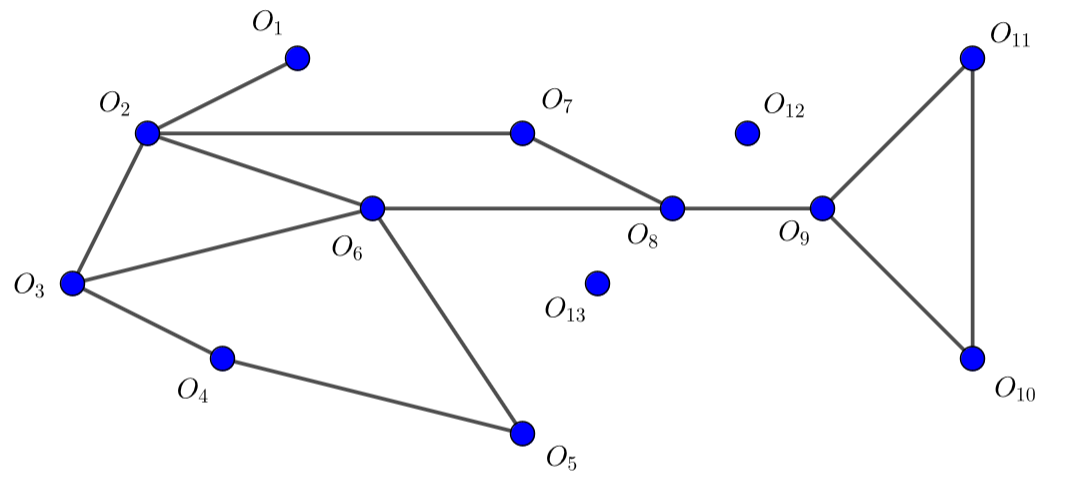
\includegraphics[width=1\textwidth]{./Images/ED01.png}
  \end{figure}
\end{frame}

\begin{frame}{Proyecciones en $\ell$-eje}
  Realicemos las proyecciones correspondientes en $X$

  \begin{figure}  
    \centering
    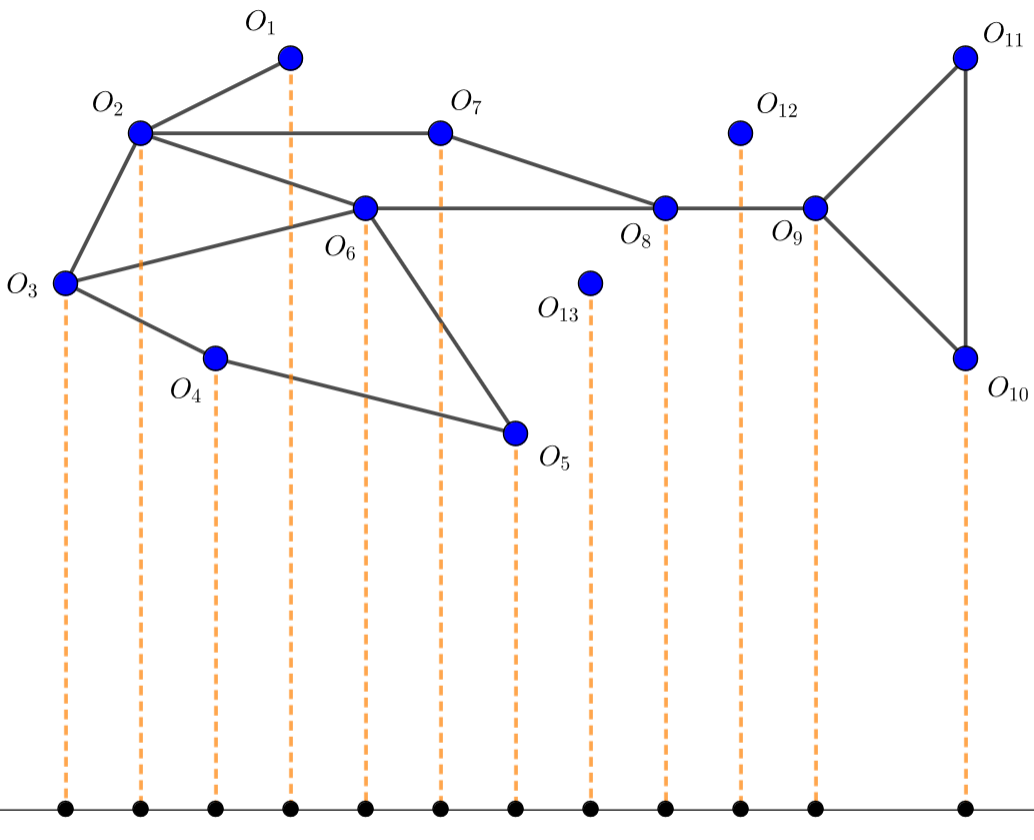
\includegraphics[width=0.8\textwidth]{./Images/ED02.png}
  \end{figure}
\end{frame}

\begin{frame}{Construcción del árbol de rangos}
  A continuación realizamos la construcción de un árbol de rangos

  \begin{figure}  
    \centering
    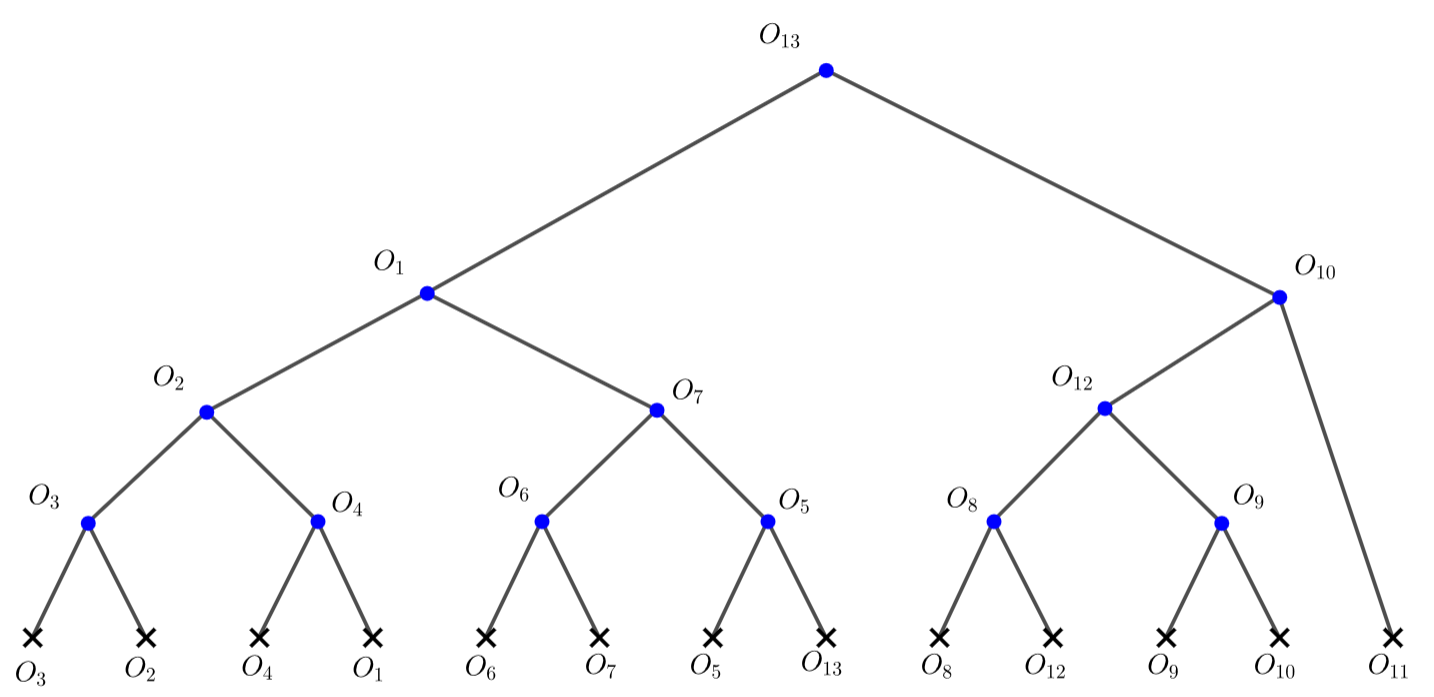
\includegraphics[width=1\textwidth]{./Images/Range1.png}
  \end{figure}
\end{frame}


\begin{frame}{...}
  Sea $T_1$ el árbol asociado a los discos en $S_1$

  \begin{figure}  
    \centering
    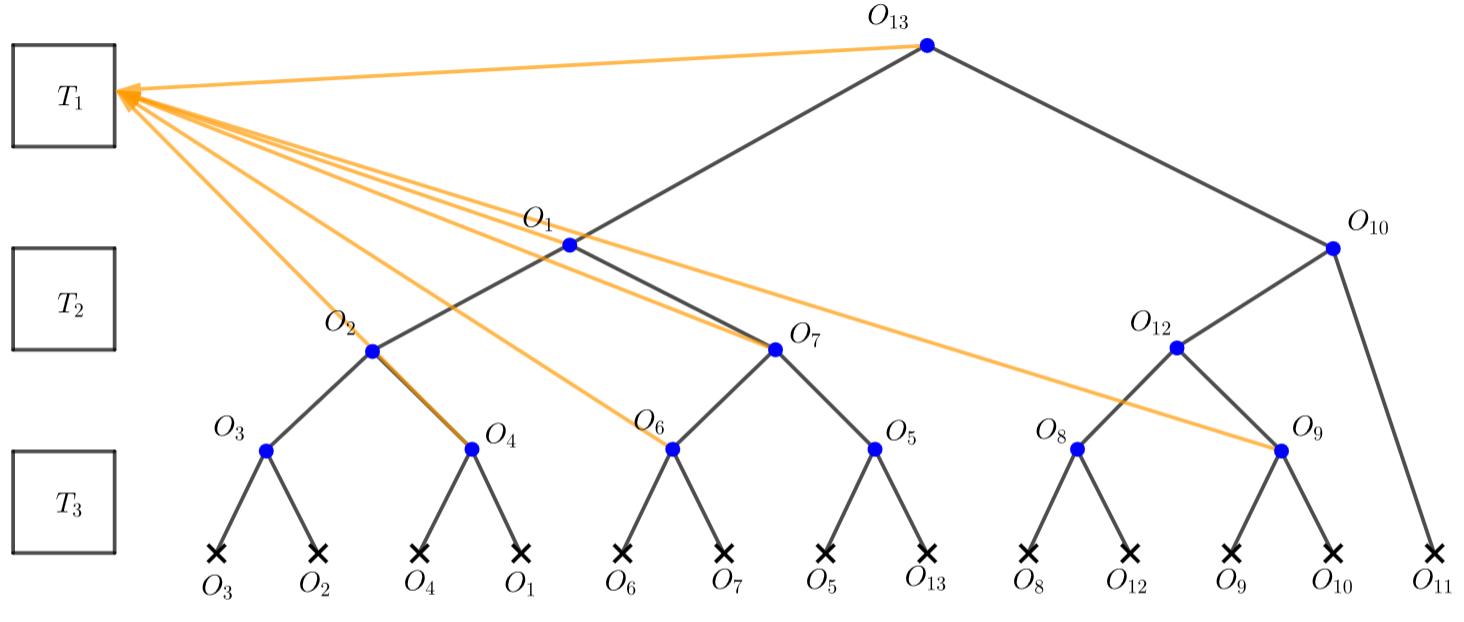
\includegraphics[width=1\textwidth]{./Images/Range2.png}
  \end{figure}
\end{frame}

\begin{frame}{...}
  Sea $T_2$ el árbol asociado a los discos en $S_2$

  \begin{figure}  
    \centering
    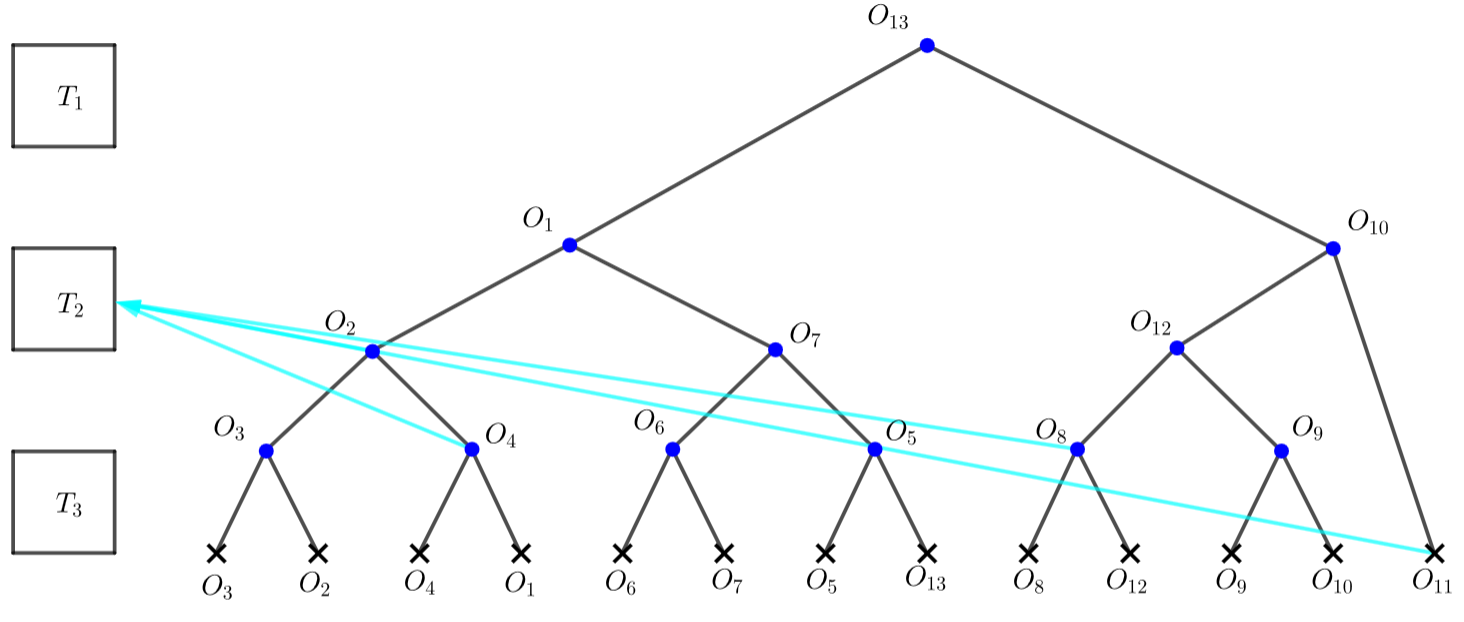
\includegraphics[width=1\textwidth]{./Images/Range3.png}
  \end{figure}
\end{frame}

\begin{frame}{...}
  Sea $T_3$ el árbol asociado a los discos en $S_3$

  \begin{figure}  
    \centering
    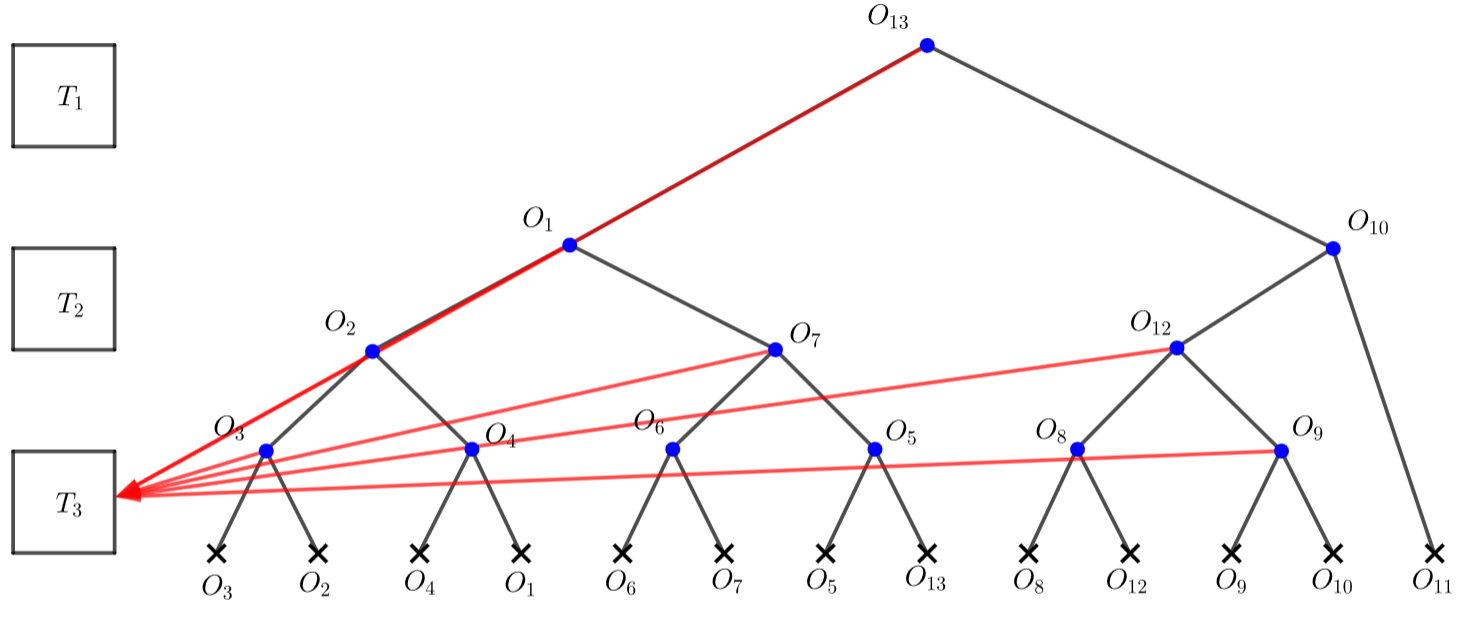
\includegraphics[width=1\textwidth]{./Images/Range4.png}
  \end{figure}
\end{frame}


\begin{frame}
  Comentarios sobre generalizaciones ...
\end{frame}

\subsection{Detalles con el algoritmo MIX.}
\subsection{Generalización a dimensiones superiores.}
%----------------------------------------------
%\mysection{¿Discos de radio dinámico?}
%\subsection{Modificaciones en la malla.}
%----------------------------------------------
\pagestyle{empty}
\Ending{¡Gracias!} % Thank You Page

% uncomment next line to include references
% \References

\end{document}
